\documentclass[12pt]{article}

\usepackage[margin=1in]{geometry}  % set the margins to 1in on all sides
\usepackage{graphicx}              % to include figures
\usepackage{amsmath, bm}               % great math stuff
\usepackage{amsfonts}              % for blackboard bold, etc
\usepackage{amsthm}                % better theorem environments
\usepackage{hyperref}

\newcommand{\kron}{\raisebox{1pt}{\ensuremath{\:\otimes\:}}} 
\newcommand{\lgamma}{\text{lgamma}} 
\newcommand{\digamma}{\text{digamma}} 

\begin{document}

\nocite{*}

\title{Calibrating the pollen-vegetation relationship}

\author{Andria Dawson}

\maketitle

\section{Introduction}

Understanding forest ecosystems of the past can provide us with
valuable information about how ecosystems respond to biotic and
abiotic factors. In particular, mapping forests back through time
offers new information not only about the climate-forest relationship,
but also forest-atmosphere interactions. In order to quantify forest
ecosystem change through time, we need spatio-temporal data. There is
no forest data that extends back through the last several millenia,
but there is a wealth of paleo-data, including fossil pollen data,
that serves as a proxy for surrounding vegetation. To make use of this
data to estimate past forest composition relies on our ability to
quantify the pollen-vegetation relationship. 

The complexity of the pollen-vegetation relationship has made it a
long-studied question in the paleoecological literature. Different
taxa produce different amounts of pollen, and XXX Describe some of the
research here....

Sampling to quantify pollen-vegetation relationships usually involves
collecting surface sediment samples to obtain pollen counts at the
time of sampling, as well as a survey of vegetation composition and
abundance of the surrounding forests. Inference can then be made about
processes that affect pollen production, dispersal, and deposition,
but only for the time of sampling. Due to widespread land-use change,
it is likely that these relationships have not remained static back
through time.

Here we use the awesome PLS data set...

To calibration the pollen-veg relationship against the PLS forest
composition data set requires that we identify pollen samples that
date back to pre-settlement. Raw fossil pollen data records depths and
counts. Usually there are additional radiocarbon dates for some number
of macrofossils scattered along the cores, not necessarily aligned
with sampled depths. These radiocarbon dates constrain age estimates,
and although radiocarbon dating facilities do assign dating errors, it
is important to keep in mind that macrofossil dates may not be exactly
aligned with dates of sediment pollen from the same depth
\cite{XXX}. To infer age as a function of depth requires an age-depth
model, although there is no consensus on the most appropriate
model. Recently, the community has recognized that importance of
estimating uncertainty, and a Bayesian age-depth model coined Bacon
developed by \cite{XXX }which does just that has gained momentum.
  
In addition to radiocarbon dates, other constraining geological
markers can often be identified from looking at stratigraphic plots of
pollen proportions.


In the case where samples are taken at multiple sites, pollen counts
are rarely modelled in a spatial context. Here we use a spatial
Bayesian hierarchical model of pollen counts at a network of sites
developed by \cite{XXX}.


\section{Data}

\subsection{Spatial domain}
Our study area is the upper Midwestern US, and includes Minnesota,
Wisconsin, and the upper peninsula of Michigan. The lower peninsula of
Michigan was not included because: 1) it is spatially disjoint from
the rest of the domain; and 2) the public land survey forest data is
still in the process of being digitized, so the composition data
available is incomplete.

\subsection{Tree taxa}
We focus on a subset of taxa that are of particular interest,
inlcuding the most abundant taxa and any taxa that are of specific
ecological importance. Our modelled taxa includes: Ash, Beech, Birch,
Elm, Hemlock, Maple, Oak, Pine, Spruce, Larch, as well as Other
Conifer and Other Hardwood groups which include those respective tree
types not explicitly included in the aforementioned list of taxa. This
separation of other hardwood and conifers as opposed to having a
single other group was motivated by ecological modellers who are often
interested in grouping taxa as deciduous, conifer, and deciduous
conifers. Additionally, the separation of other hardwood and conifers
allows the model to treat each group seperately and tease out inherent
differences between conifer and deciduous seed production, although we
recognize that the variability in production and dispersal within each
of these groups is still large.

\subsection{Public Land Survey (PLS) data}

%XXX Jack and Simon 
Prior to major European settlement, the US General
Land Office conducted a Public Land Survey (PLS) throughout much of
the United States in order to simplify the sale of federal
lands. Surveyors documented section location using trees as landmarks,
and recorded genus or species, diameter, and location (azimuth and
distance from corner). This data set provides a systematic survey of
the forest before settlement, and has been used by foresters,
ecologists, and historians to understand ecosystem and land-use change
through time. In the Upper Midwest, the survey was conducted during
XXXX-XXXX. Due to the slow-growing nature of temperate forests, including those in the Upper
Midwest, we can think of the PLS data as a snapshot of
forest composition in time.

%XXX Chris...  
Survey data for the Upper Midwest has been recently
digitized, and aggregated to an 8km square grid \cite{XXX}. However,
due to its sparse nature, sampling methodology, and surveyor bias the
PLS data set contains inherent variability. Here we work with a
smoothed version of the PLS data, based on a Bayesian spatial multinomial 
model \cite{XXX}.

\subsection{Pollen data}
With the push for robust and reproducible research from the scientific
community, paleoecoinformatics has responded with the development of
tools that make accessing and using large datasets possible. One such
tool that has made this work possible is the Neotoma database
(\url{neotomadb.org}; \cite{XXX}), which stores a variety of types of
paleoecological data, including pollen data. Accessing this data can
be done using the Neotoma API (), or using the R neotoma package
\cite{XXX}. Using these tools granted us access to 176 fossil pollen
cores falling within our domain.

%XXX: Jack or Simon, anything to add here about this dataset?
In addition to the data obtained from Neotoma, we also had access to a
data set belonging to Calcote, Hotckiss, XXX. This data set included
57 cores in our domain. Of these 57, 9 were long cores (analogous to
those from neotoma), while the remaining 48 had only core top and
pre-settlement samples (at least in the data file we had access to).

Associated with each of the cores is a table containing counts by
taxon for a series of depths. For each pollen core we are interested
in the pre-settlement sample that is closest in time to the PLS
data. Typically, age-depth models are used to assign ages to sample
depths. However, there are many different types of age-depth models,
each with its own set of benefits and shortcomings. Instead, we rely
on a panel of experts to interpret patterns in the pollen count data
to identify pre-settlement sample estimates. All long cores were
suitable for this exercise.

\subsection{Expert elicitation of pre-settlement depth}
Widespread land clearance that occurred during European settlement
provided habitat for certain non-arboreal colonizers, resulting in
increases in non-arboreal pollen. In the Upper Midwest, significant
increases in Ambrosia, Rumex, or Poaceae are typically coincident with
the settlement horizon. When these increases can be identified based
on pollen count data, we can determine the pre-settlement sample - the
sample that falls just before any increases in agricultural indicator
species. In practice, identifying increases in agricultural indicators
is often difficult, when possible, and can be subjective. We were
interested in: 1) identifying the pre-settlement sample using
consistent methodology, and 2) assessing the variability in assignment
of pre-settlement among analysts. To address these questions, we asked
a team of expert palynologists to identify the pre-settlement sample
for 185 pollen records (176 from Neotoma and 9 from the Calcote data
set). Experts were provided with pollen diagrams depicting
proportional changes through time as a function of depth for key
indicator species and the ten most abundant arboreal taxa. Experts
were prohibited from relying on stratigraphic dates (radiocarbon or
other) or age-depth model estimates of sample age. We also provided
space so that experts could comment on their certainty of their
pre-settlement sample. In the case that there was no distinguishable
pre-settlement sample, experts were instructed to report NA. In the
case that experts were uncertain, they were instructed to note this,
with or without justification for their uncertainty.

\section{Calibration model}

We work on a regular grid composed of 8 km square grid cells, which is
the resolution defined by the PLS data. Although the grid is composed
of discrete cells, the underlying vegetation composition is assumed to
be a smooth spatial process. Spatial cells are indexed by
$s=1,\ldots,S$, where $S=8013$.

Trees are sources of pollen - they produce and distribute pollen
across the landscape. Here, the gridded PLS data provides us with a
representation of how these trees are distributed throughout the Upper
Midwest domain. We can then think of grid cells as being producers of
pollen, and the amount of pollen produced by a given grid cell
depends on the compositional makeup of that cell (among other things). 

Pollen produced by vegetation within each grid cell can be deposited
locally within that same grid cell, or farther away in other grid
cells. The proportion of pollen produced in a focal cell
deposited in that same cell is defined by $\gamma$, while the
remaining $1-\gamma$ is dispersed into the neighborhood around that
grid cell. For a focal grid cell $s_i$, the pollen produced by taxon
$p$ within that cell that remains local is described by

\begin{align}
\gamma \phi_p r_p(s_i)
\end{align} 

where $\gamma$ is the proportion of pollen that is deposited locally,
$\phi_p$ is the scaling factor that accounts for differential
production, and $r_p(s_i)$ is the proportional abundance of vegetation
in $s_i$.

The remaining proportion ($1-\gamma$) of pollen produced in $s_i$ is
dispersed to other grid cells according to an isotropic dispersal
kernel centered at $s_i$. The dispersal kernel weights all pollen
dispersing away from the focal cell as a function of the distance from
$s_i$ to any neighboring cell $s_k$ by $w(s_i, s_k)$. Here $w(s_i,
s_k)$, is defined to be a gaussian dispersal kernel written as
\begin{align}
w(s_i, s_k) = \exp\left( - \frac{d(s_i, s_k)^2}{\psi^2} \right),
\end{align}
where $d(s_i,s_k)$ defines the distance between cells $s_i$ and $s_k$
and $\psi$ is a parameter that describes the spread of the kernel. As
expected, the weight assigned by this kernel is a decreasing function
of distance - less pollen is distributed farther away.

%Previous work has shown that pollen dispersal distances can reach up to XXXX, and that long-distance dispersal events may be rare, but have the ability to drive range expansion XXX.
 
We can then define the pollen produced by taxon $p$ dispersing from
$s_i$ to $s_k$ by
\begin{align}
\frac{1}{C} (1-\gamma) \phi_p r_p(s_i) w(s_i, s_k),
\end{align}
where $C$ is a normalizing constant equal to the sum of the weights of
all the cells to which pollen can be dispersed, defined be a
rectangular region that covers and extends beyond the limits of the domain.

%% An anisotropic kernel may better approximate true pollen dispersal due to prevailing winds, although prevailing wind direction in the Upper Midwest is not constant throughout the domain due to the proximity to the great lakes, making the inclusion of this asymmetry complicated. %

%and therefore including this non-constant asymmetry in the modeling framework is not straightforward. 

So far we have described the model from a source-based perspective,
describing how pollen produced in grid cells is dispersed. However, we
really want to model the pollen arriving at the grid cell in which a
pond lies $s(i)$. To do this, we simply sum all the contributions that
have been dispersed to $s(i)$, which includes both the locally
deposited pollen plus the pollen dispersed to $s(i)$ from all other
grid cells. Therefore the pollen from taxon $p$ arriving at $s(i)$ is
given by

\begin{align}
\gamma \phi_p r(s(i)) + \frac{1}{C} (1-\gamma) \phi \sum_{s_k \neq s(i) } r(s_k) w(s(i), s_k).
\label{eq:arriving}
\end{align}

Finally, pollen counts at pond $i$, denoted by $\bm{y}_i$, are
modelled using the dirichlet-multinomial to account overdispersion
resulting from the sparsity and uneven distribution of sampled lakes
throughout the domain. We have
\begin{align}
\bm{y}_i \sim DM (n_i, \alpha_i)
\label{eq:DM}
\end{align}
where the precision parameter $\alpha_i$ is equal to the sum of \ref{eq:arriving} over all taxa
\begin{align}
\alpha_i = \sum_{p=1}^K \gamma \phi_p r(s(i)) + \frac{1}{C} (1-\gamma) \phi \sum_{s_k \neq s(i) } r(s_k) w(s(i), s_k).
\label{eq:arriving}
\end{align}

\subsection{Numerical implementation}

Due to the non-conjugate nature of the multivariate likelihood terms,
we are relegated to using MCMC methods. With the goal of achieving
more efficient sampling with respect to the effective sample size per
unit time, we used the Stan statistical modeling software to estimate
parameters. Stan implements a variant of the Hamiltonian Monte Carlo
method called the No-U-Turn Sampler. HMC is a gradient based sampling
method, which uses these directional derivatives to make informed
decisions about how to move along (and sample from) the joint
posterior surface. HMC can be more efficient that a traditional MCMC
in many cases, but requires additional tuning that is difficult to
perform in practice, as well as user defined gradients that can be
difficult to impossible to compute analytically. NUTS overcomes the
tuning issues by extending the HMC algorithm to including automatic
tuning. Stan provides an implementation of the NUTS sampler that uses
automatic differentiation to compute model gradients, making the
sampler accessible to anyone able to program their model using a
bugs-like syntax.

\section{Results}

\subsection{Expert elicitation of pre-settlement depth}

Four experts participated in the elicitation exercise. For 59 out of
185 sites, the experts were in total agreement: they all identified
the same pre-settlement sample. The remaining sites varied in level of
disagreement - in 79 cases, experts identified two pre-settlement
samples; in 38 cases there were 3 pre-settlement samples identified;
and in 4 cases there was no agreement. Without further analysis, these
results confirm our assumption that identification of biostratigraphic
markers is subject to variability between analysts. For 4 of the sites
for which there was complete agreement, all experts chose not to
identify a pre-settlement sample. Two of these sites were at Rice
Lake, which is an anomalous site overwhelmed by a Zizania and Poaceae
signal, and does not show any indication of settlement.

Based on these results, we were faced with the challenge of
determining site suitability for inclusion in our calibration data
set. Ideally, the pre-settlement sample uncertainty would be included
into the modelling framework. However, this elicitation exercise
varies from those that are typically conducted to construct priors;
here we are uncertain about our data, and not our parameters. Instead
of increasing the complexity of the statistical model, we first screen
for site suitability, and then for all suitable sites base our
pre-settlement sample assignment on the expert determinations.

There were 11 sites for which 3 or 4 experts did not assign a
pre-settlement sample, and these were considered unsuitable for
calibration. We think about this as there being no majority consensus
regarding the existence of a land-clearance signal. As a second pass
filter, we looked to existing age models associated with our pollen
cores. Ages for the identified pre-settlement depths were compared to
1850, which serves as an approximate year of settlement in the upper
midwest (although we recognize that settlement year in quite variable
even within the midwest).  Although uncertainty associated with age
models can be large, there is also a tendency to identify patterns
when in fact there are none \cite{XXX}. There were seven sites for
which two experts chose not to assign a pre-settlement sample while
the remaining two chose depths with modelled ages that were 500 years
away from 1850 were discarded.

After completion of the elicitation exercise, a more thorough
examination of the stratigraphic data used to calibrate age models, we
noticed that several cores had core tops with dates much older than
expected. Further investigation revealed that three of the cores
included in our analysis were missing core tops. Core tops for both
Lake Mary and Green Lake pre-date settlement, and therefore were
discarded. The third core for Lake Kotiranta had a core top
corresponding to the pre-settlement sample, and was retained for
inclusion in the calibration data set. Interestingly, for each of
these cores, 1-3 experts identified a pre-settlement sample (although
under the assumption that the uppermost sample was in fact a surface
sample).

The addition 48 cores in the Calcote data set were not candidates for
the elicitation exercise because they had only a core top and a
pre-settlement sample recorded. We comtemplated their inclusion in our
calibration data set because their pre-settlement samples are
identified using different methodology (and analyst) than the
remaining sites. We opted to include these samples, based on our
confidence in the data set/analyst and the recognition that including
these sites would result in a substantive increase to our sample size.

After suitability screening, we were left with 165 long cores plus 48
additional short cores, for a total of 213 cores in the calibration data set.

\subsection{Exploratory data analysis}

To visually assess the relationship between sediment pollen and tree
taxa, we compare pie maps showing the proportions of each taxon
throughout space (Figure~\ref{XXX}). If the patterns here were
identical, then knowing the proportions of vegetation and sediment
pollen would be identical (i.e. a 1:1 relationship). Although the
patterns we do see are consistent, there are some striking
differences. First, we see that pine dominates the pollen records for
much of the northern half of the domain, while it is present but
relatively less abundant in the PLS data. Second, we see areas that
have higher relative abundances of Hemlock, Tamarack, and Maple. There
are more subtle differences in the less abundant taxa. These
differences indicate that as expected, the relationship between
sediment pollen and vegetation is complex. Note that the PLS pie map
represents an aggregated version of the 8km gridded dataset, and that
this coarsened data set is used for exploratory purposes only (pies
would not be visible if the original scale were used).

To better assess spatial distributions of pollen versus PLS data, we plot the data as heat maps by taxon. Differences in these extent of these distributions are indicative of successful pollen dispersal. For example, for both Birch and Pine, we see that the distributions of sediment pollen extend beyond the boundaries of those shown in the PLS data \ref{XXX}.

\subsection{Modelling results}

Three chains were run for with a warmp-up of 250 iterations, followed
by a sampling period of 10,000 iterations. Warm-up iterations were not
used in further analysis. For a total of 30,000 iterations, the
effective sample size of the joint log posterior was XXX. Trace plots
for the joint log posterior show the efficient mixing achieved by the
sampler \ref{XXX}.

Parameter estimates from the calibration model run allow us to
quantify the relationship between the sediment pollen and the
vegetation on the landscape. In particular, we are interested in
learning whether sediment pollen from a network of sites can be used
as a proxy for vegetation at large spatial scale. An intuitive way to
think about the pollen-vegetation relationship is to plot the
proportion of sediment pollen against the proportion of vegetation, by
taxon. We know this relationship is complicated, and the hope is that
the calibration model allows us to better predict sediment pollen than
if we tried to predict based on data alone. In Figure~\ref{XXX}, we
plot the proportional relationship between raw pollen and vegetation,
and raw pollen and predicted pollen, considering only the focal grid
cell to which the ponds belongs. More specifically, the predicted
pollen is obtained by scaling the focal cell vegetation data by
$\phi$. The relationship between the raw pollen and vegetation is
clearly not 1:1. In particular, we see that some taxa, such as beech,
maple, other conifer, and tamarack, are not prolific pollen producers
- they can appear in large proportions on the landscape, but do never
appear in large proportion in the pollen record. (Note that it could
also have been the case that the produced pollen may have been
abundant, but travelled elsewhere.) We also point out that some
relationships are difficult to identify, for example pine, where the
taxon may be relatively sparse to abundant on the local landscape, but
this relative abundance does not provide much insight to the relative
abundance in the pollen record. Although in some cases the model
appears to account for some of the processes governing the
pollen-vegetation relationship and shifts the raw versus predicted
pollen points closer to the 1:1 line, there is still something
missing.

In Figure~\ref{XXX}, we again plot raw pollen against the vegetation
or predicted pollen by taxon, but here the predicted pollen is based
on the local plus non-local predictions obtained from the full
calibration model. Now that dispersal has been accounted for, we see
that the raw versus predicted pollen points fall more closely along
the 1:1 line. This indicates that the model is accounting for some of
the processes that take the pollen from the tree to the sediment, and
that the model predictions are an improvements to predictions based on
data along.

XXX There are several cases where the model does not do a good job accounting for the model   

Taxon-specific estimates for the production/dispersal parameter $\phi$
form three distinct groups in $\phi$ parameter space, that: low,
intermediate, and high $\phi$ or production/dispersal. The group of
taxa with low production/dispersal are Hemlock, Beech, Maple, Other
Conifer, and Tamarack. This low production/dispersal pattern is
evident in Figure~\ref{fig:preds}, where the representation of these
taxa in the pollen records is consistently less than their
representation on the landscape (except in a few anomalous cases). The
high production/dispersal group includes pine and birch, which can
also be seen in Figure~\ref{fig:preds} by their propensity to be
over-represented in the pollen record relative to the landscape. All
other taxa fall into the intermediate production/dispersal
group. These results agree in generel with estimates of the
pollen-vegetation relationship based on sites in Wisconsin and the
Upper Peninsula of Michigan found by \cite{prentice1986}. In that
work, Pine and Birch had the largest slopes (top
producers/dispersers), and maple and tamarack as limited
producers/dispersers. \cite{jackson1990} also found that Pine and
Birch were good dispersers with effective source areas of ~1000m,
while Maple was found to have a much smaller source area indicating
limited dispersal.

The local versus non-local weight $\gamma$ was estimated to have a
mean of $0.20\,(0.19, 0.22)$. This indicates that 20\% of the pollen
produced by vegetation in a focal grid cell is deposited in that grid
cell, while the remaining 80\% disperses elsewhere in the domain. The
dispersal kernel specifies the weights that determines where the
pollen goes, and depends on the spread parameter $\psi$ which was
estimated to be $210\,(200, 220)$ km. This implies that 50\% of the
pollen produced in a focal cell is deposited within 140 km of the
focal cell, and 90\% is deposited within 296 km of the focal cell \ref{fig:dvd}.

To assess our assumption that all taxa share a dispersal kernel with
spread controlled by the scalar $\psi$, we re-ran the model letting
$\psi$ vary by taxon. All taxon-specific 95\% credible intervals had
some overlap with the credible intervals for the single-$\psi$ case,
except for Maple, Other hardwood, and Tamarack
(Figure~\ref{fig:psi_vary_psi}). On average, Maple had by far the
largest value of $\psi$, followed by Other hardwood, which implies
that these two taxonomic groups are disperse the farthest. However,
the 95\% credible interval for $\psi$ for Maple was wide, and in both
cases the increased value of $\psi$ corresponded with an increased
value of $\phi$ relative to the single-$\psi$ runs
(Figure~\ref{fig:phi_vary_psi}). This indicates that there may be
some issues with parameter identifiability inherent in the model when
we allow $\psi$ to vary by taxon, and as such results from this run
should be interepreted with caution.

To visualize the dispersal patterns predicted by our model, we can estimate deposited pollen for each grid cell in the domain (previously we were estimating deposited pollen only at lakes for which we had pollen data). When we compare these maps of relative pollen abundance with those depicting the relative tree abundance, we see that the model predicts 

\section{Discussion}

XXX

%% \section{Acknowledgements}

%% XXX


% %map showing core locations
% \begin{figure}
% \centering
% 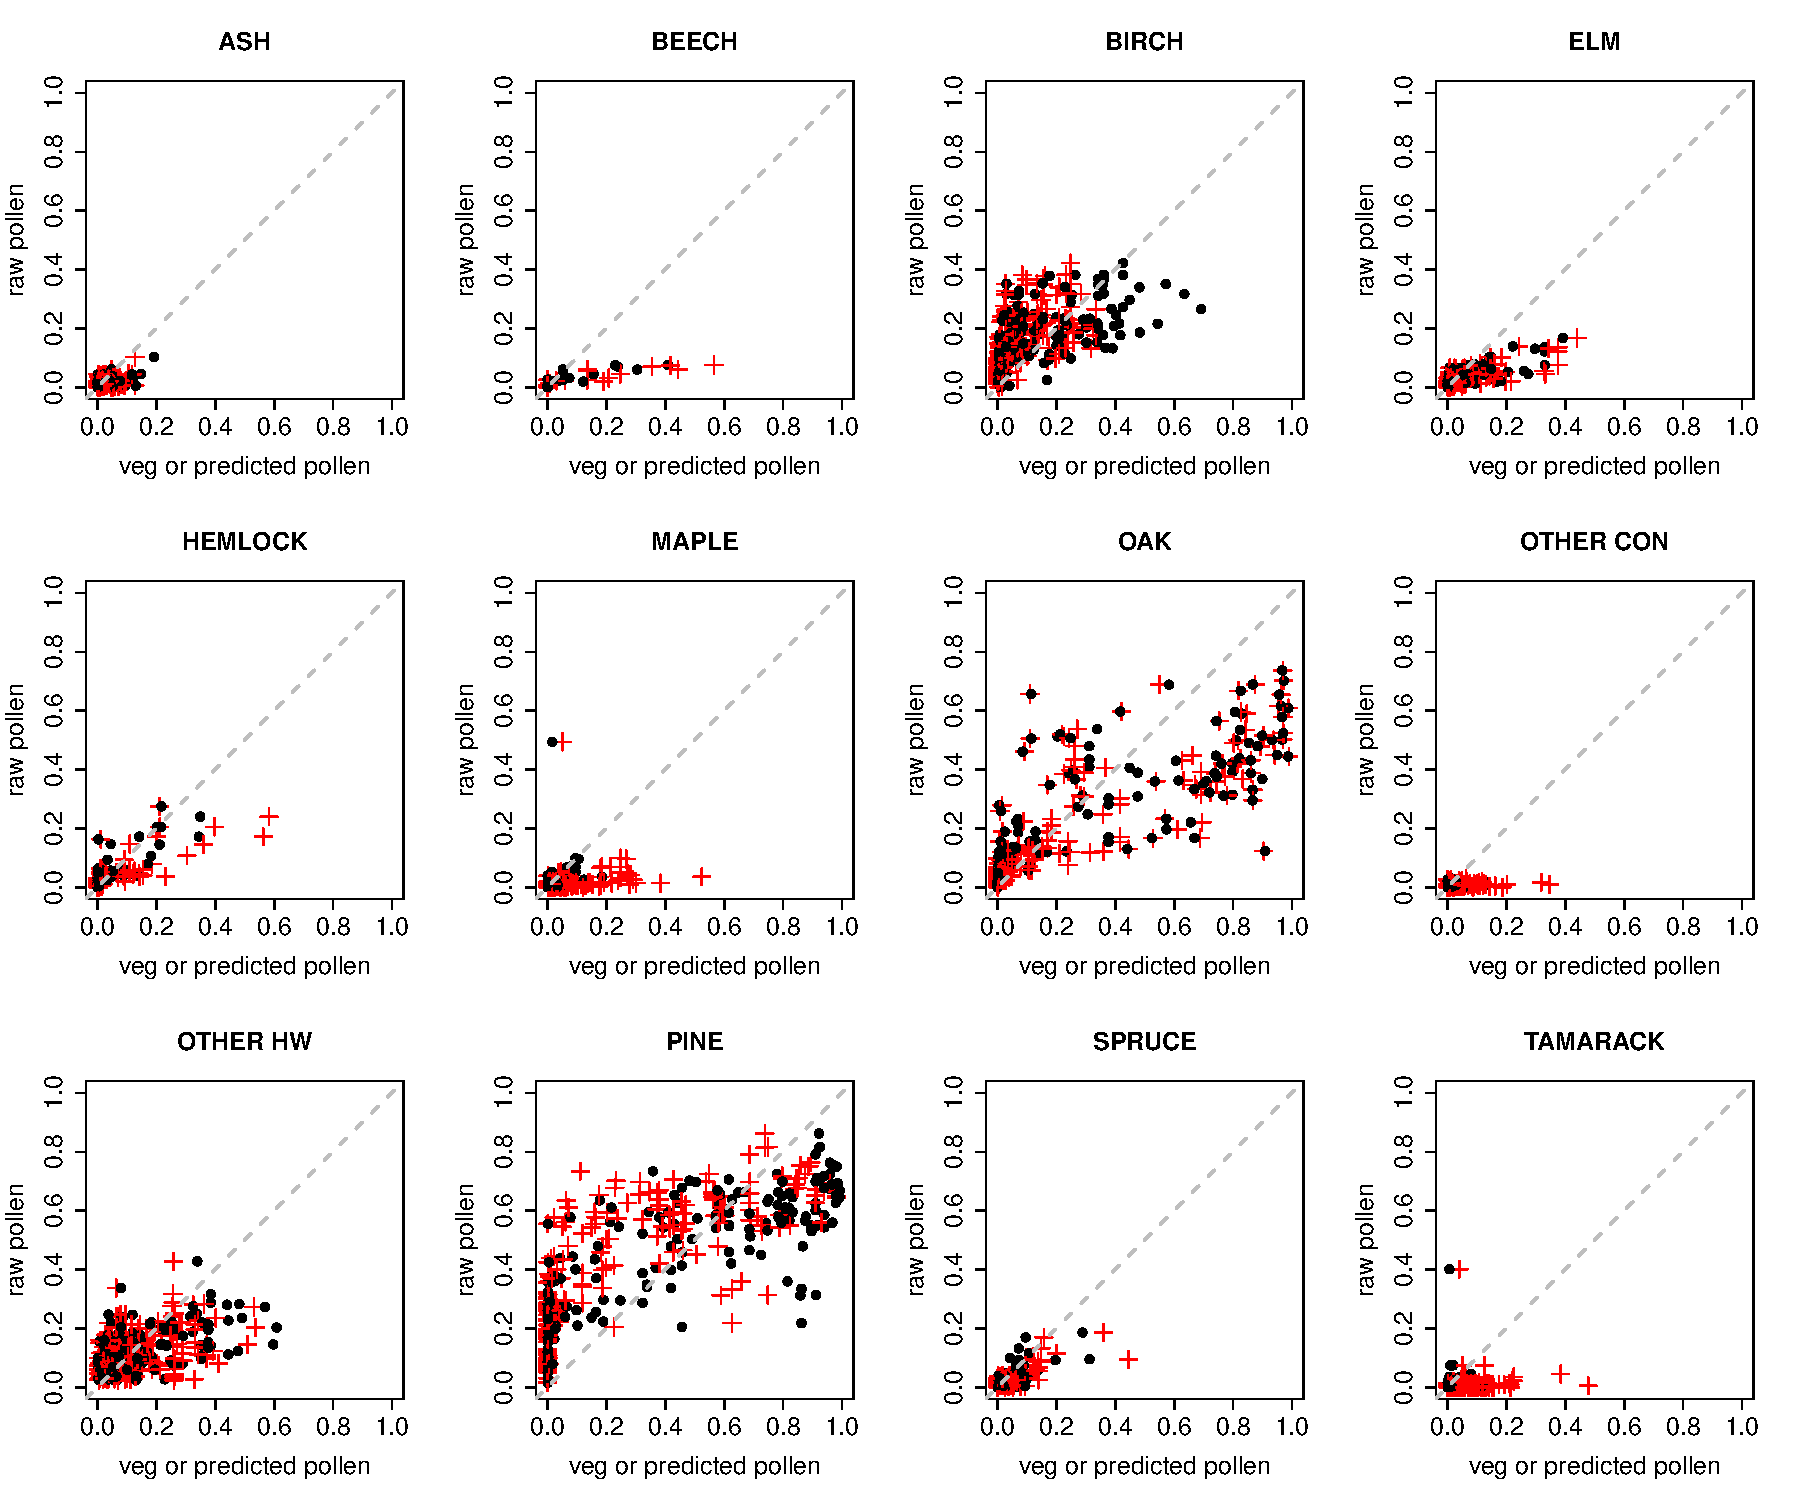
\includegraphics[width=7in]{figures/pollen_focal_scaled.pdf}
% \caption{}
% \label{fig:focal_scaled}
% \end{figure}

%PLS and pollen pie maps
\begin{figure}
\centering
\begin{tabular}{c}
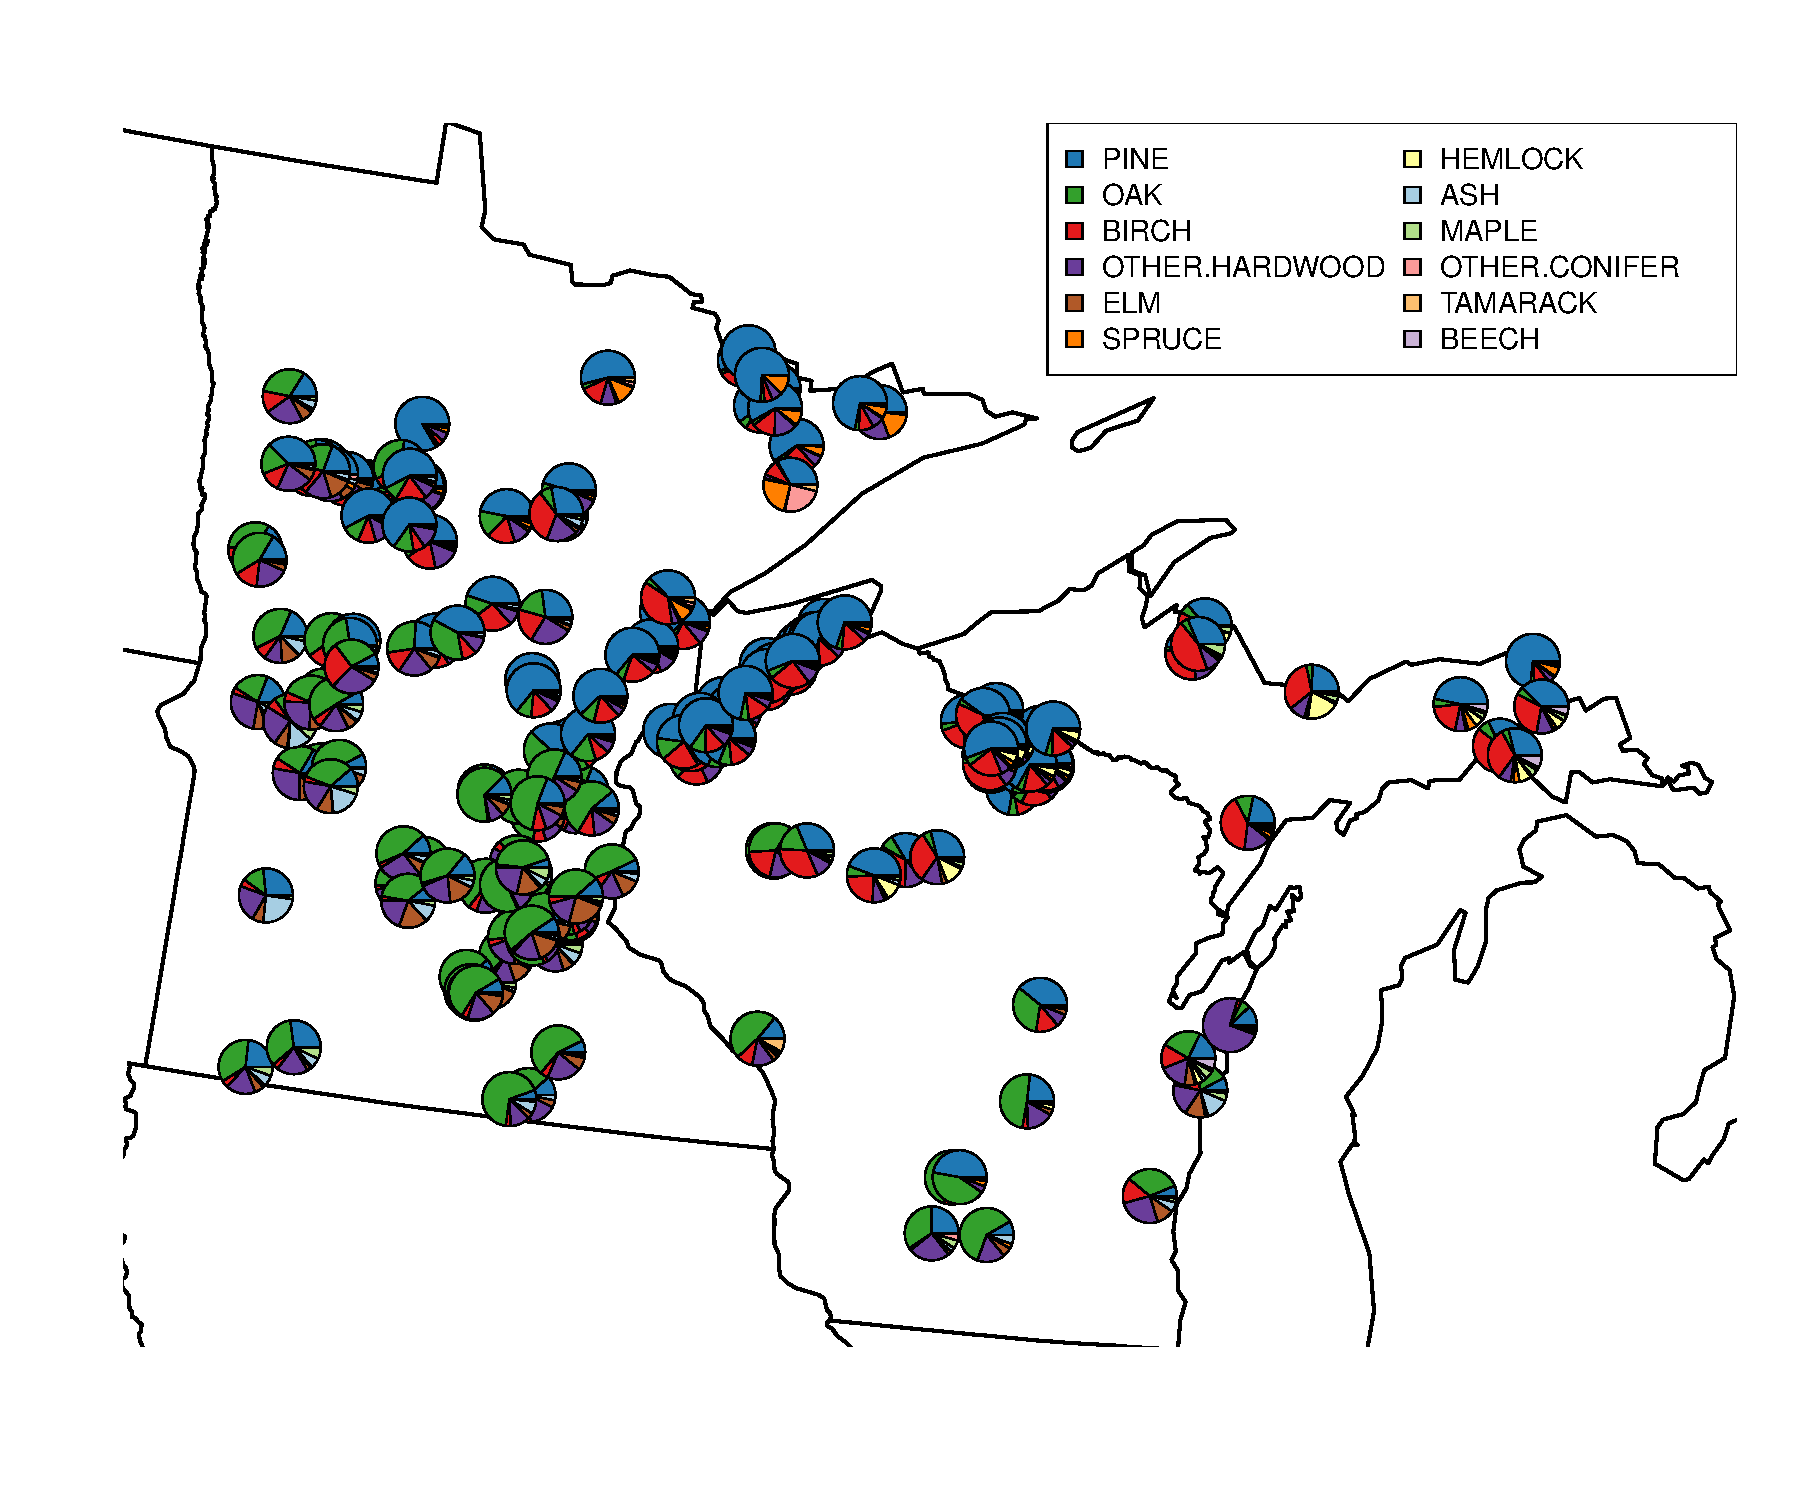
\includegraphics[width=5in]{figures/pie_plot_pollen_UMW_v01.pdf} \\
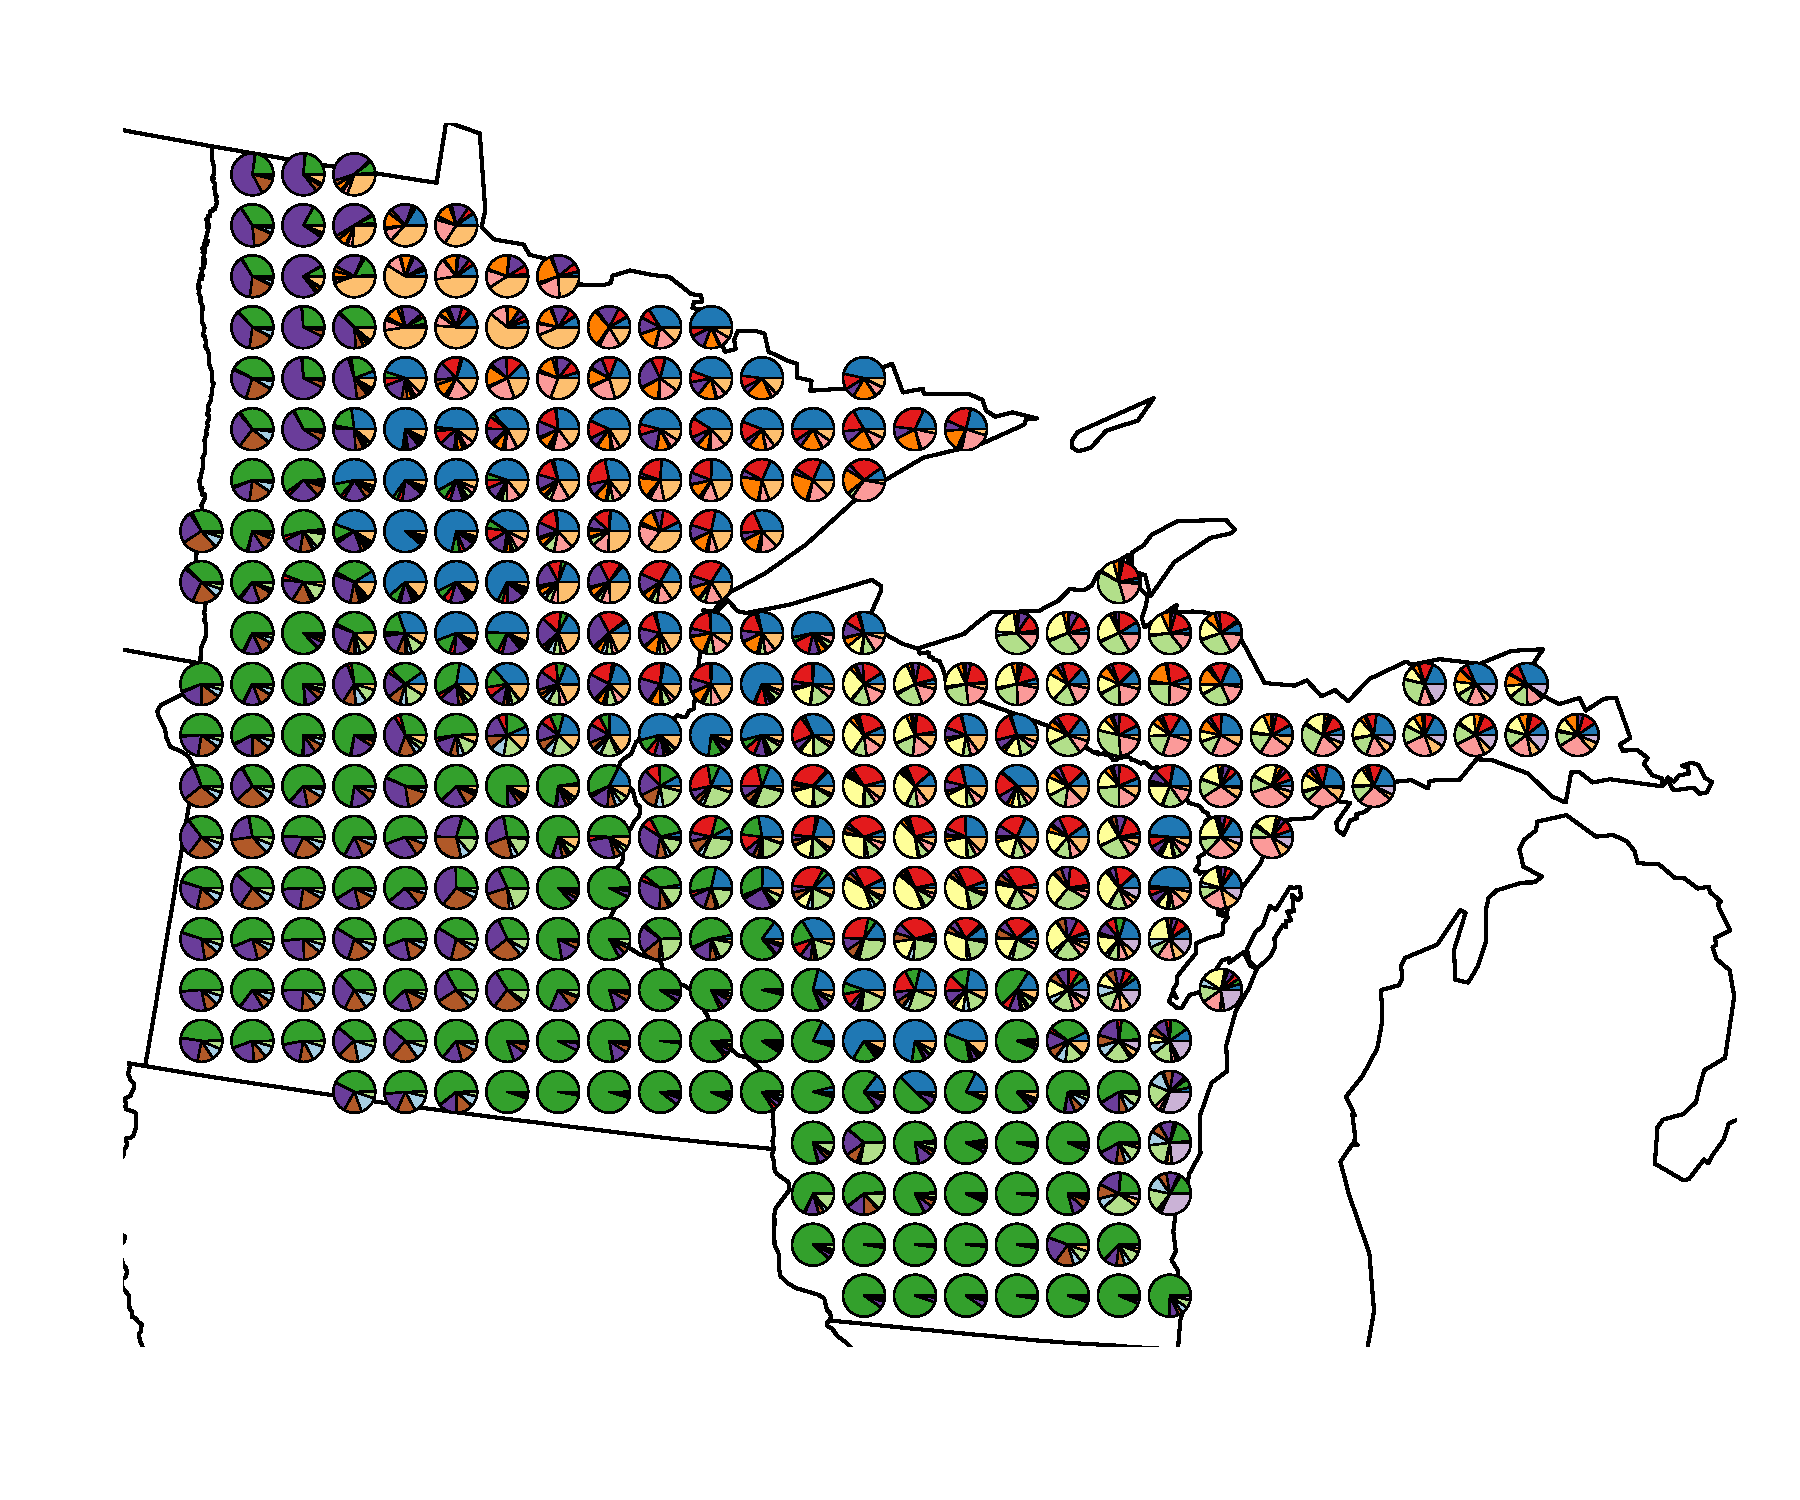
\includegraphics[width=5in]{figures/pie_plot_pls_UMW_v01.pdf}
\end{tabular}
\caption{Pie maps depicting the relative composition of pollen (top)
  and PLS vegetation (bottom) from the data. Note that the PLS data
  has been aggregated to a coarser resolution for illustrative
  purposes.}
\label{fig:pie}
\end{figure}

%veg and pollen heat maps: pine
\begin{figure}
\centering
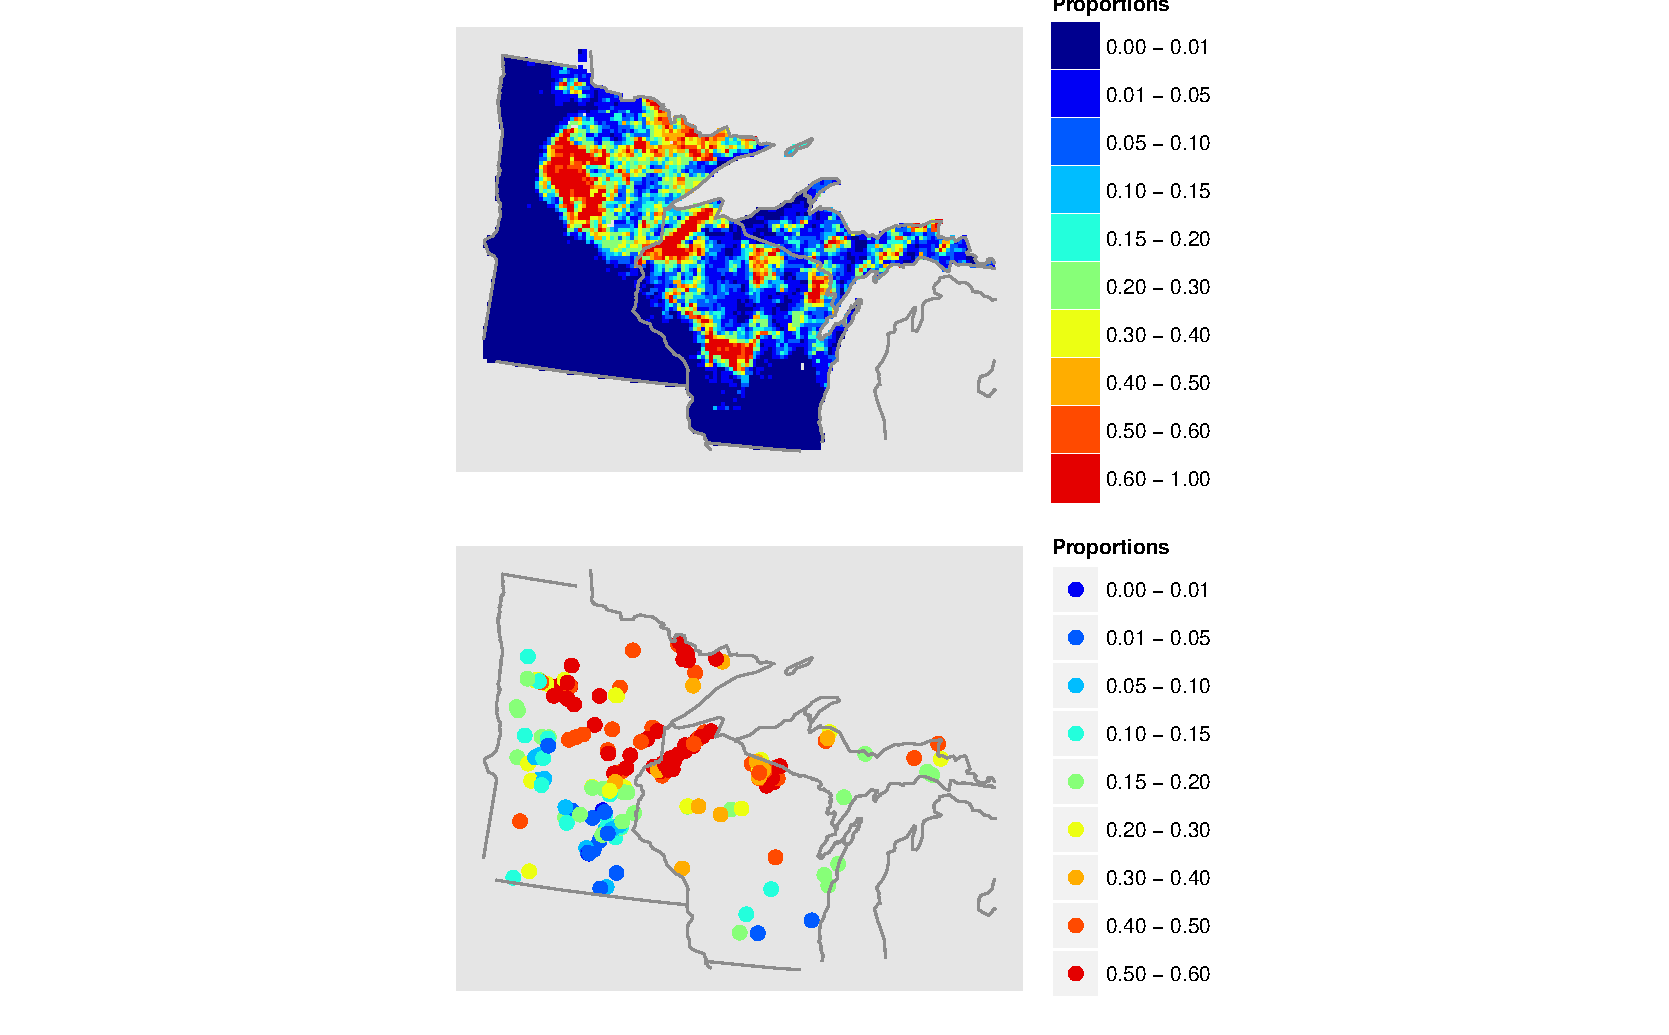
\includegraphics[width=7in]{figures/maps_compare_PINE.pdf}
\caption{Heat maps showing the range limits of Pine in the PLS composition data (top) and the sediment pollen (bottom).}
\label{fig:compare_maps_PINE}
\end{figure}

%veg and pollen heat maps: birch
\begin{figure}
\centering
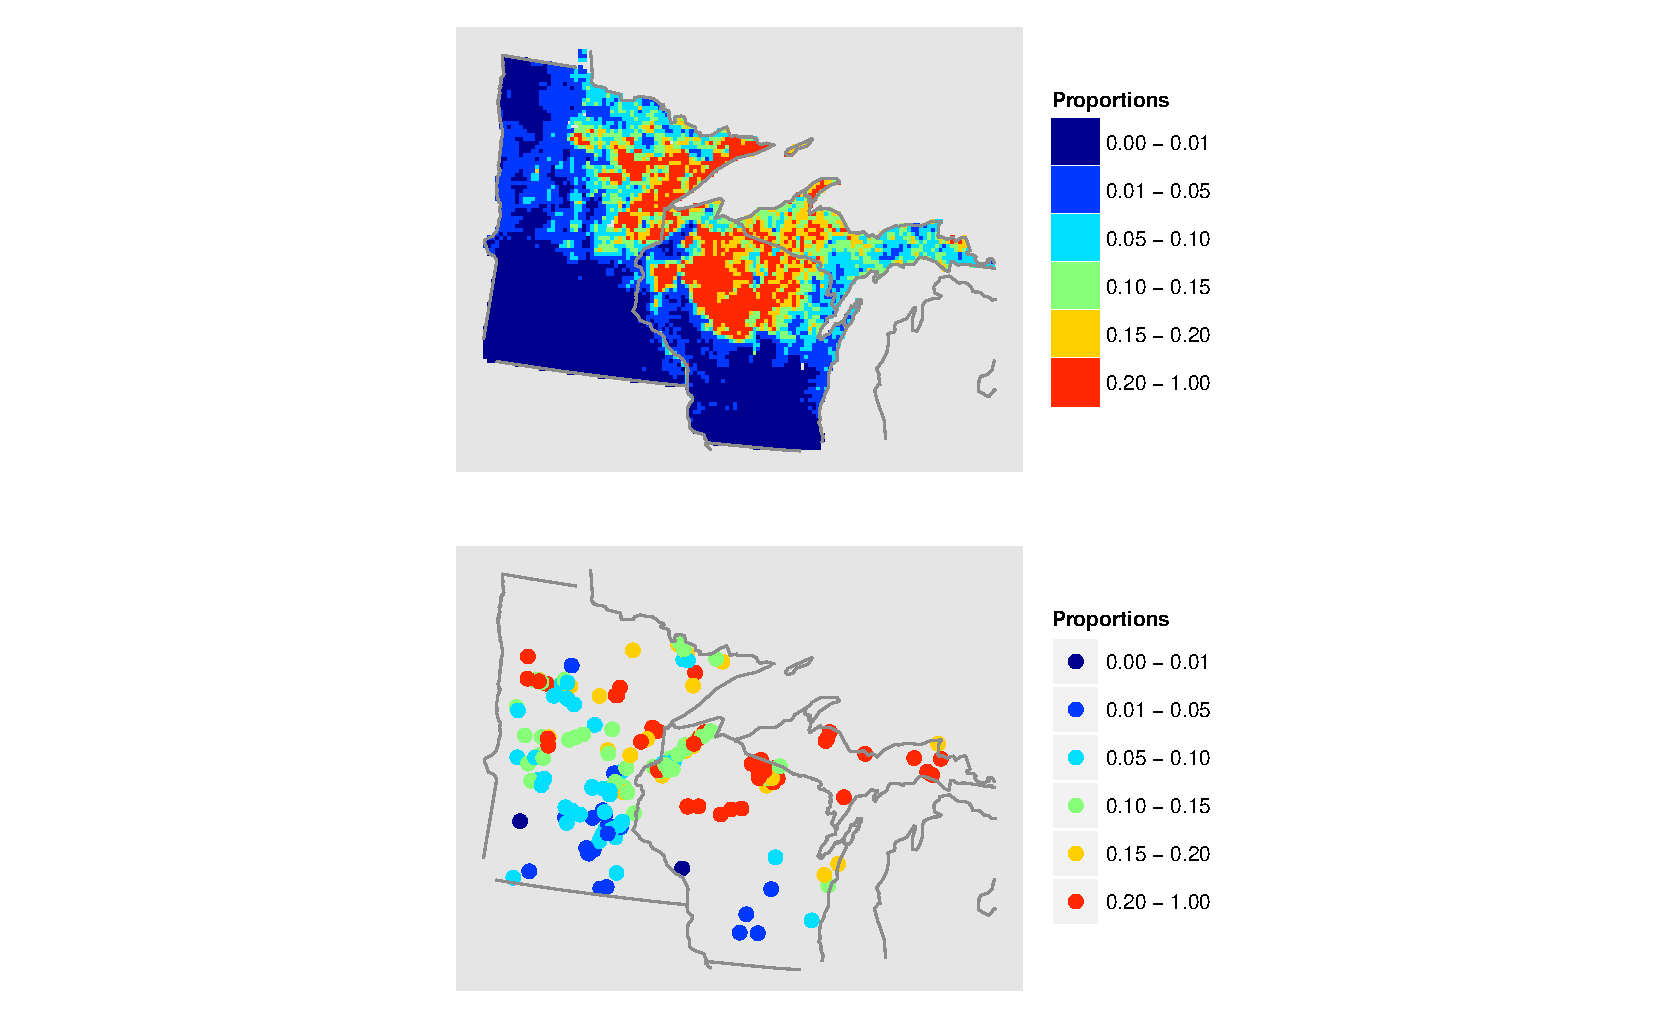
\includegraphics[width=7in]{figures/maps_compare_BIRCH.pdf}
\caption{Heat maps showing the range limits of Birch in the PLS composition data (top) and the sediment pollen (bottom)}
\label{fig:compare_maps_PINE}
\end{figure}

%pollen raw versus scaled focal
\begin{figure}
\centering
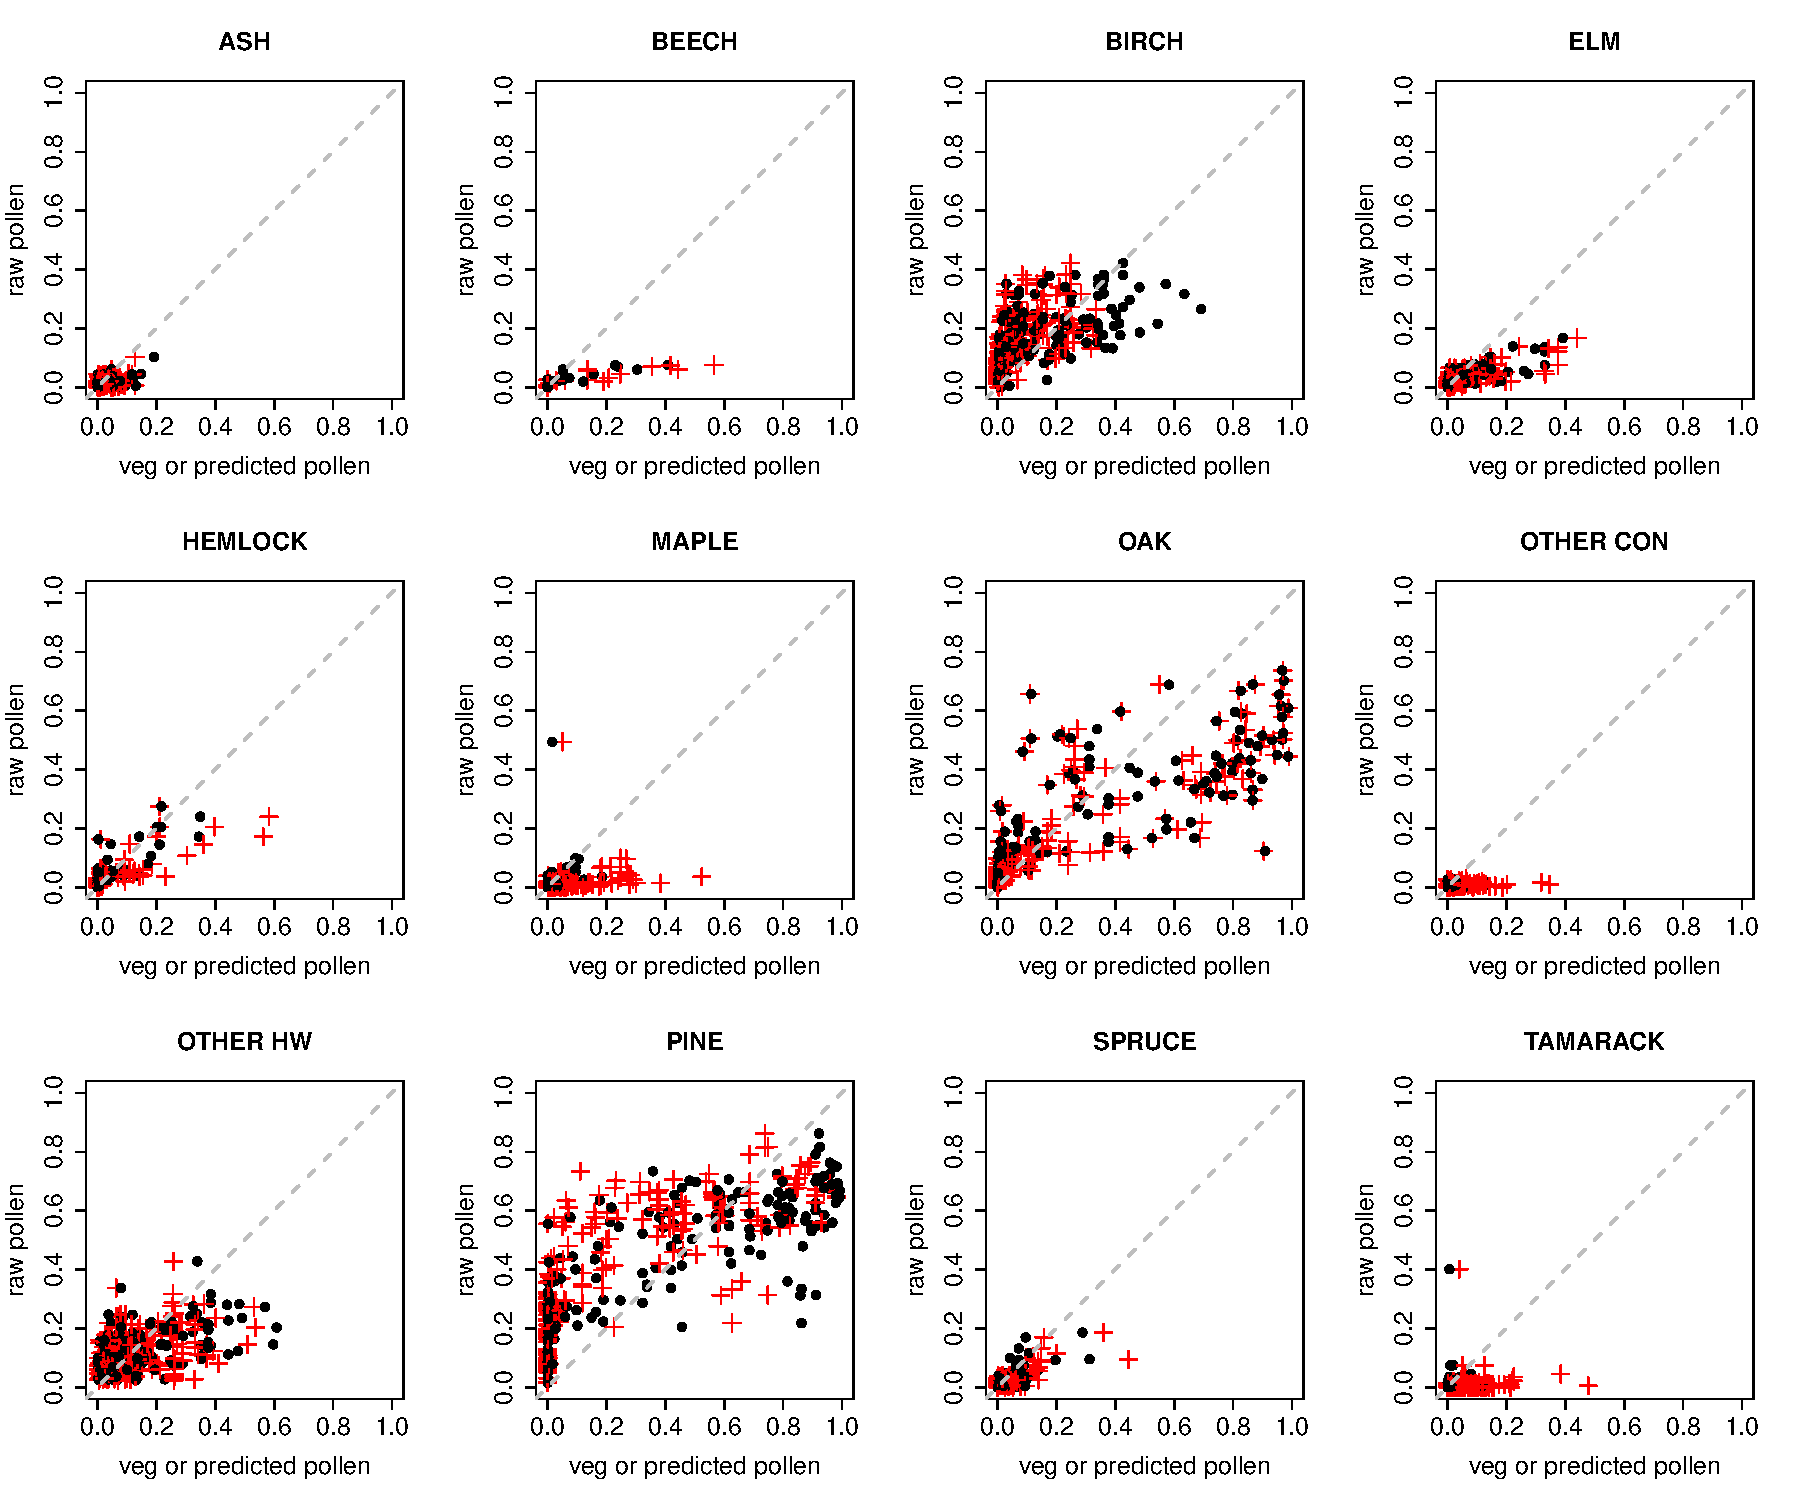
\includegraphics[width=7in]{figures/pollen_focal_scaled.pdf}
\caption{Pollen proportions plotted against local vegetation proportions (red crosses) or local vegetation proportion scaled by $\phi$ (black dots), by taxon.}
\label{fig:focal_scaled}
\end{figure}

%pollen raw versus predicted
\begin{figure}
\centering
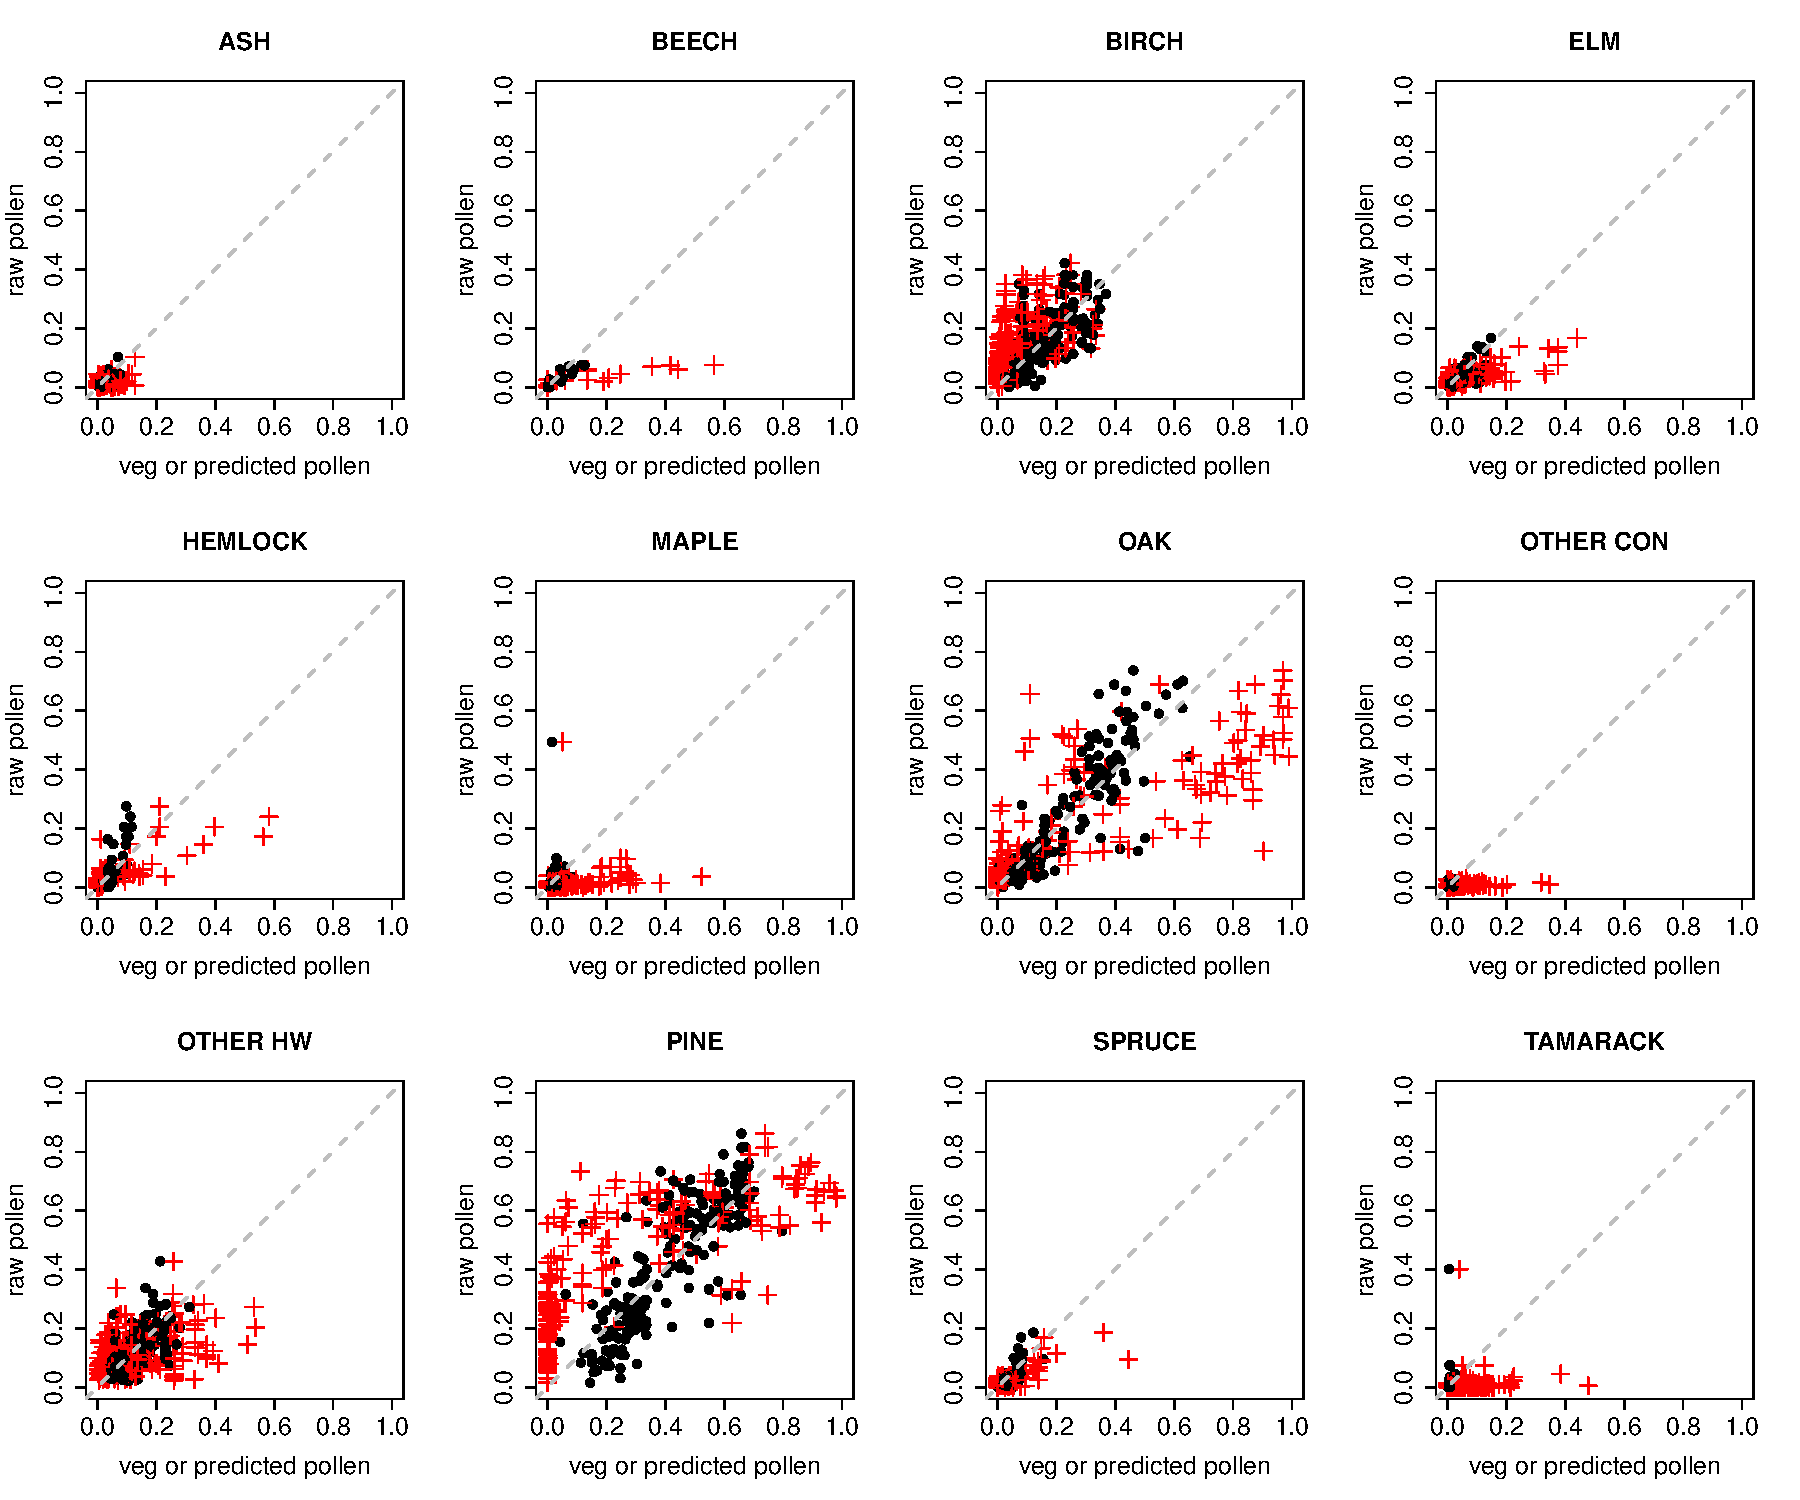
\includegraphics[width=7in]{figures/pollen_preds.pdf}
\caption{Pollen proportions plotted against local vegetation proportions (red crosses) or model-predicted pollen (black dots), by taxon.}
\label{fig:preds}
\end{figure}

%phi (differential production)
\begin{figure}
\centering
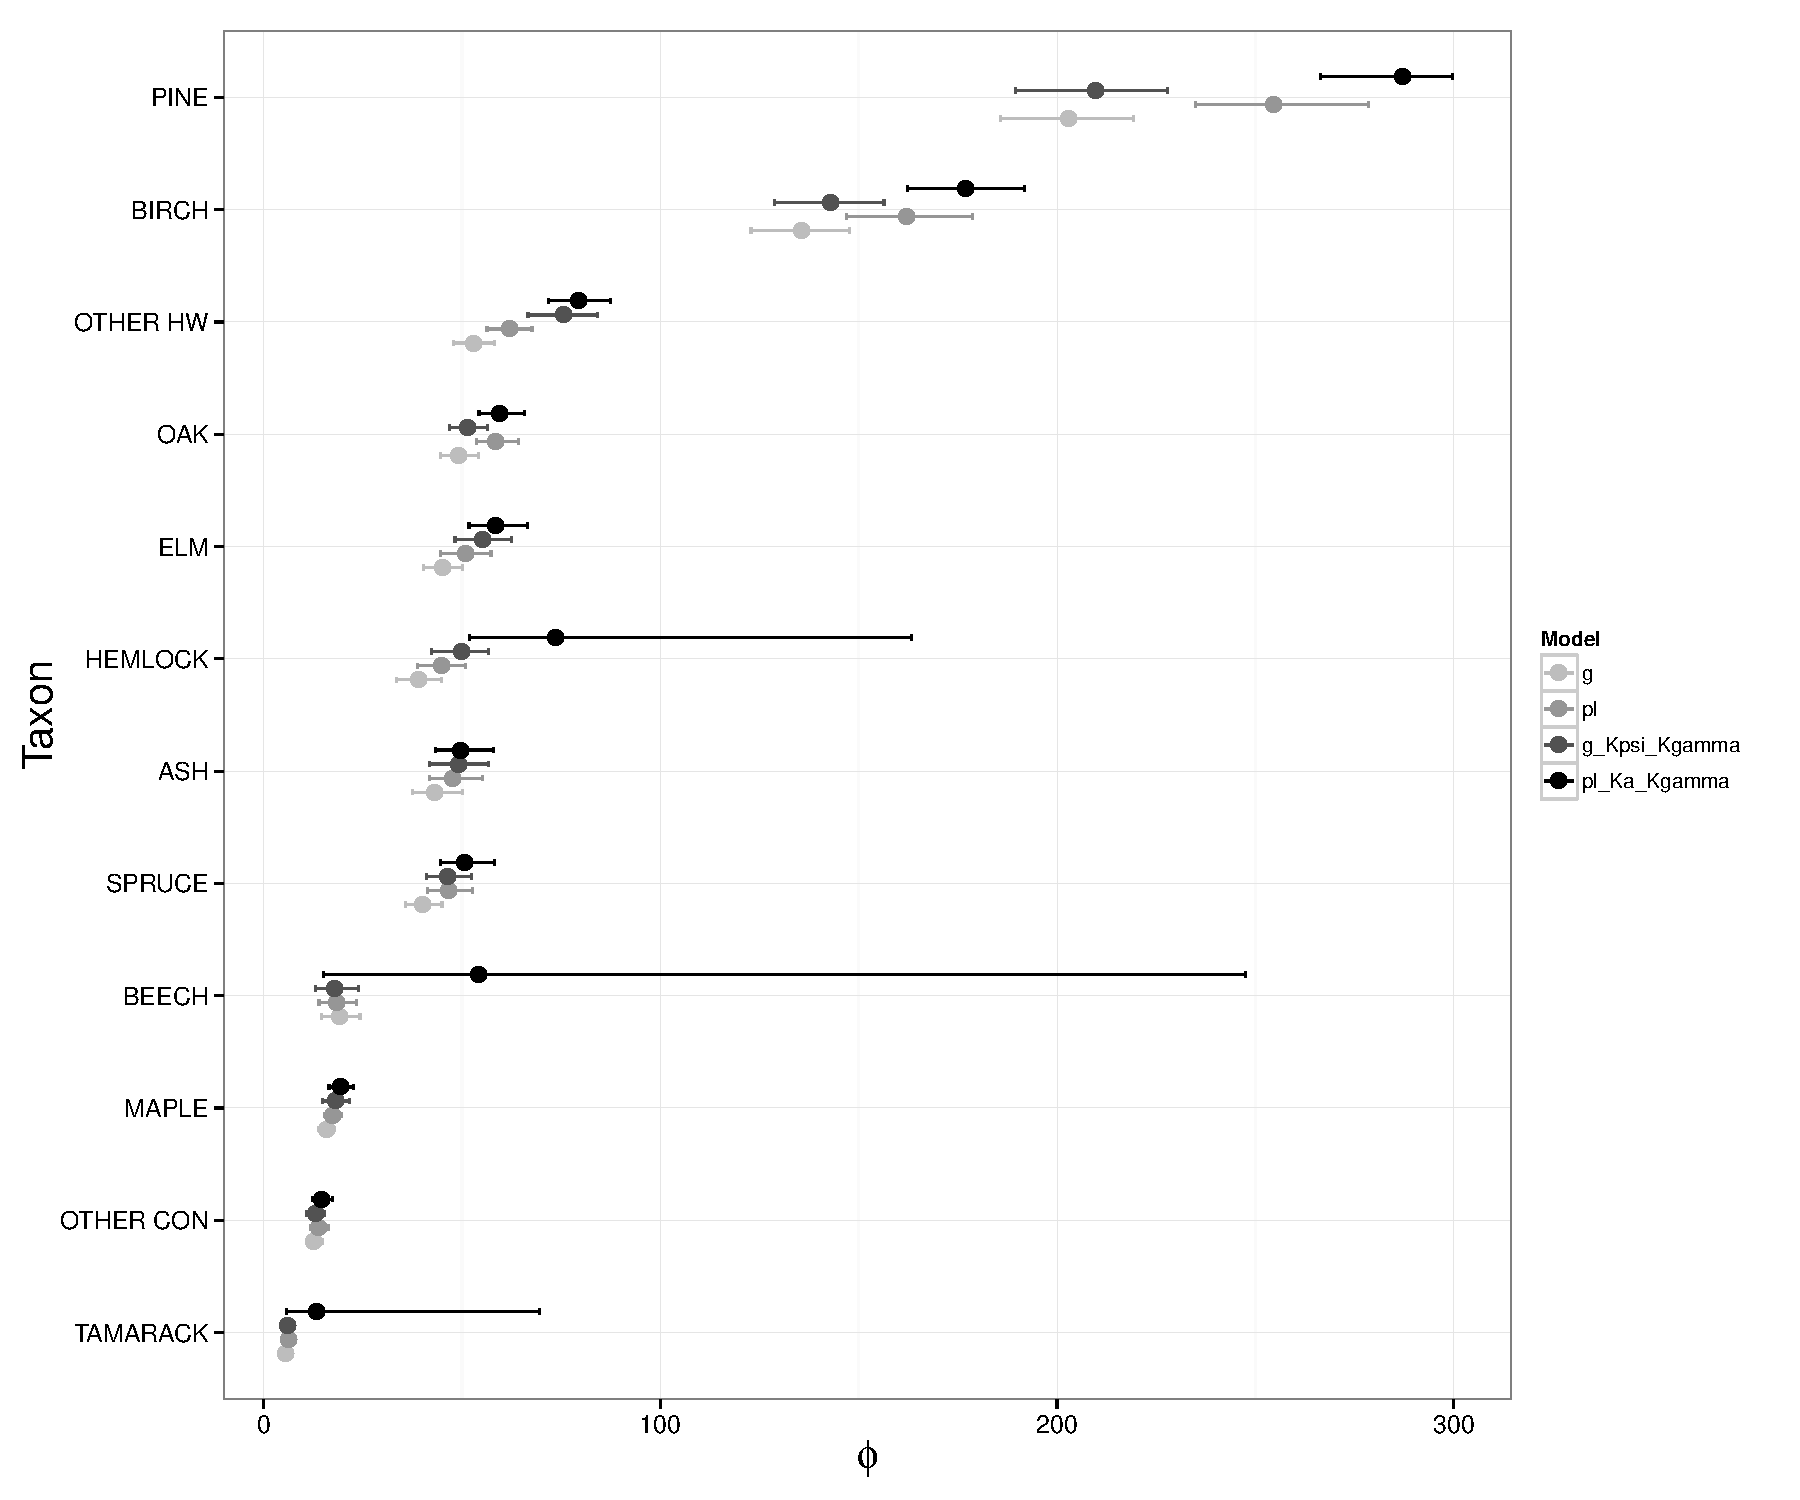
\includegraphics[width=7in]{figures/phi.pdf}
\caption{Mean values and 95\% credible intervals for the estimated values of the differential production parameter $\phi$.}
\label{fig:phi}
\end{figure}

%proportion pollen versus radius
\begin{figure}
\centering
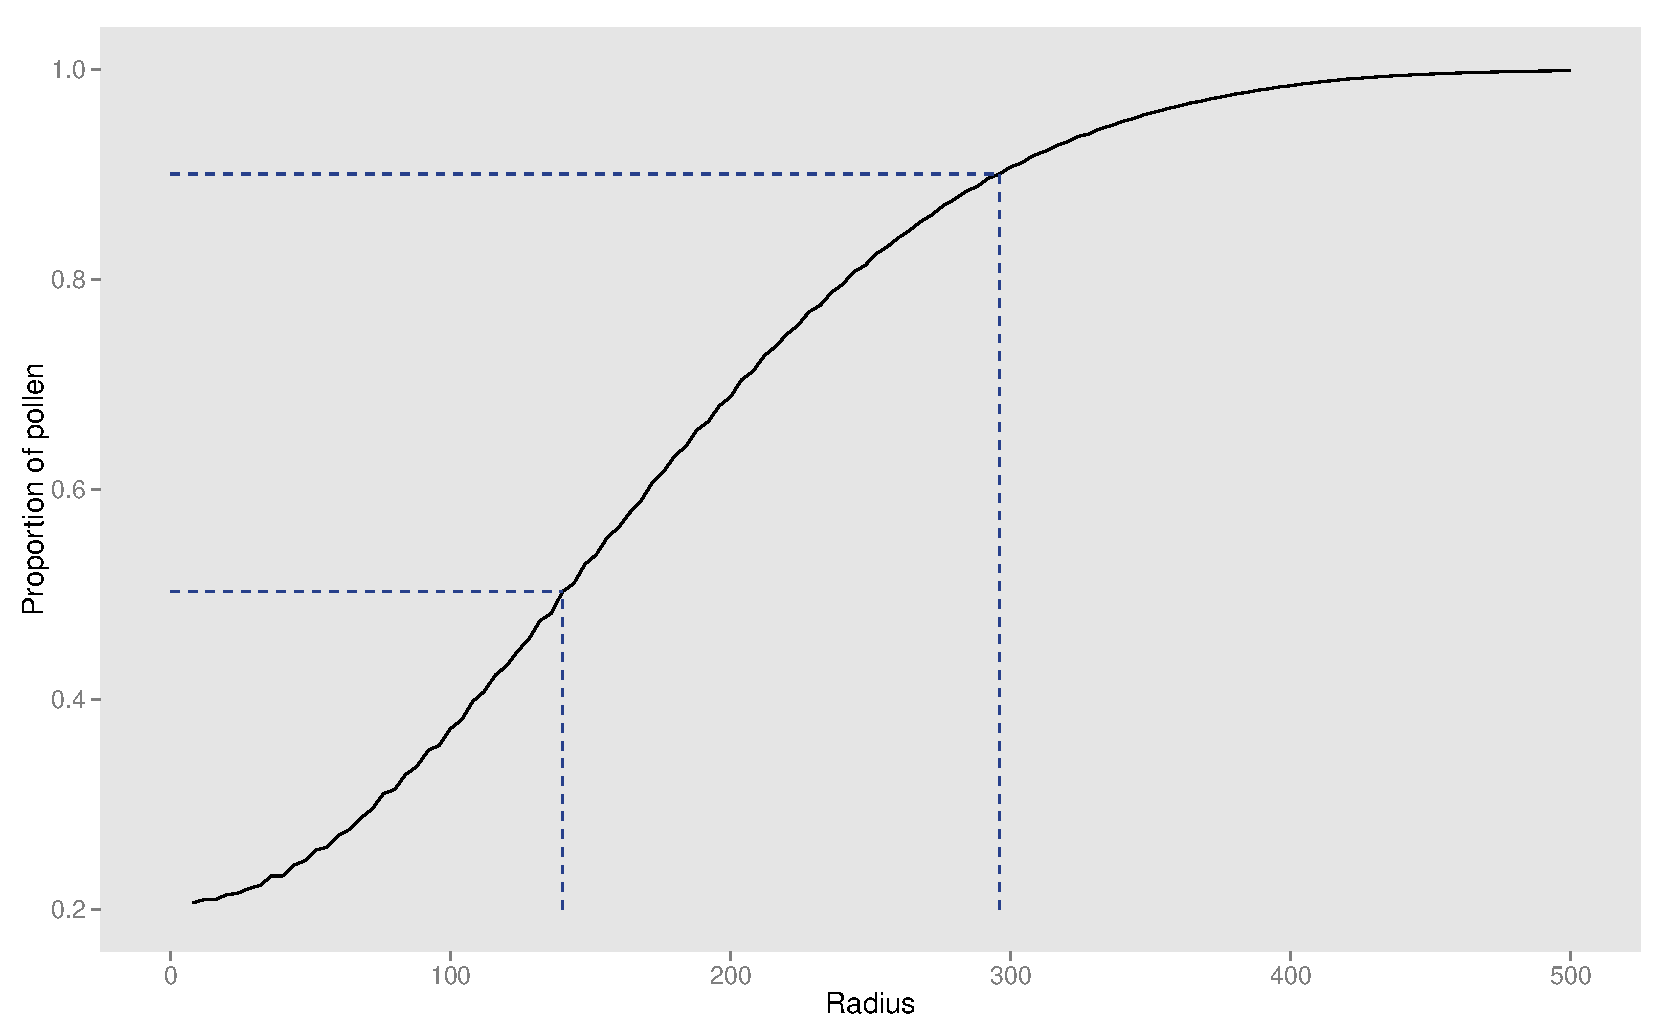
\includegraphics[width=7in]{figures/dispersal_vs_distance.pdf}
\caption{Here we consider pollen produced by a focal cell, and plot the proportion of deposited pollen as a function of the radius of a circle centered at the focal cell.}
\label{fig:dvd}
\end{figure}

%psi: vary psi case
\begin{figure}
\centering
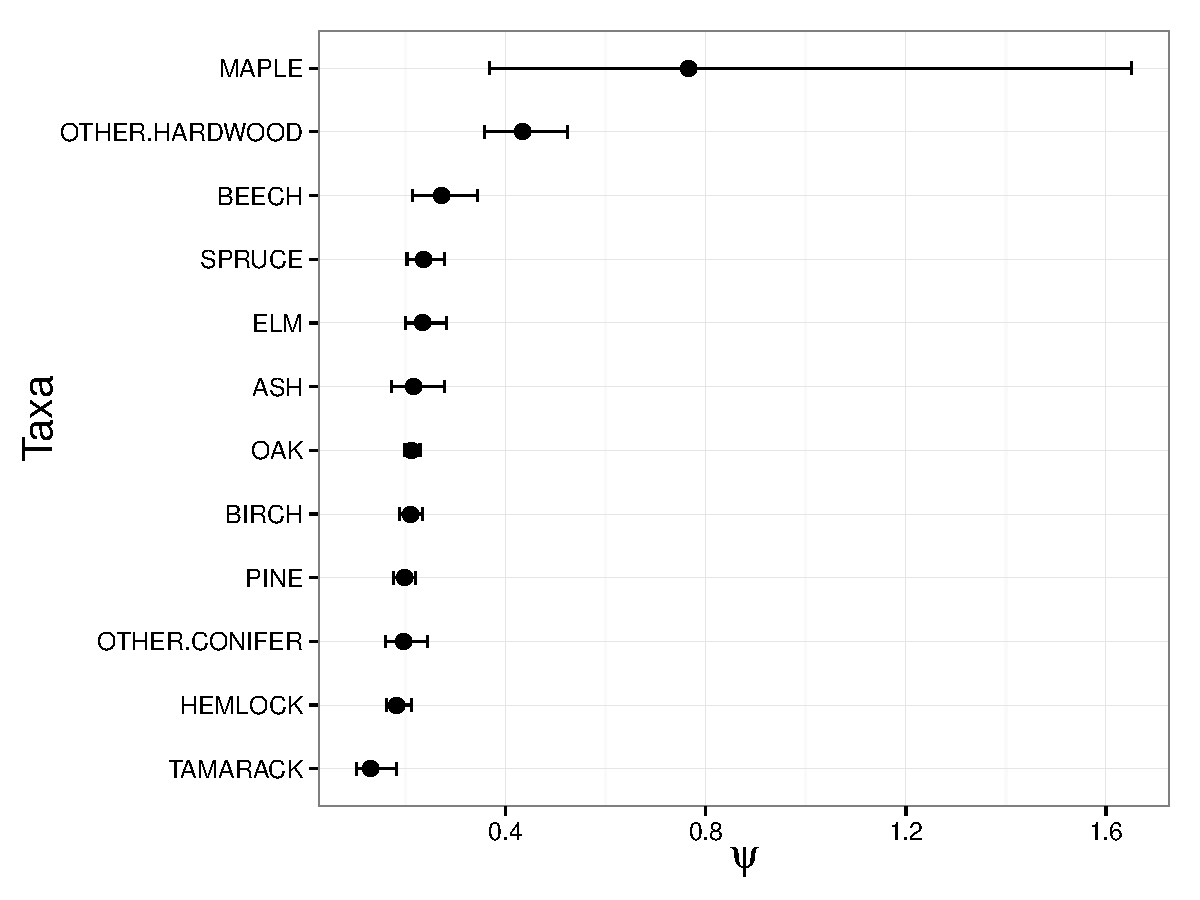
\includegraphics[width=7in]{figures/psi_vary_psi.pdf}
\caption{Mean values of 95\% credible intervals for the estimated values of the dispersal kernel spread $\psi$ for the case where we let $\psi$ vary by taxon.}
\label{fig:psi_vary_psi}
\end{figure}

%phi: vary phi case
\begin{figure}
\centering
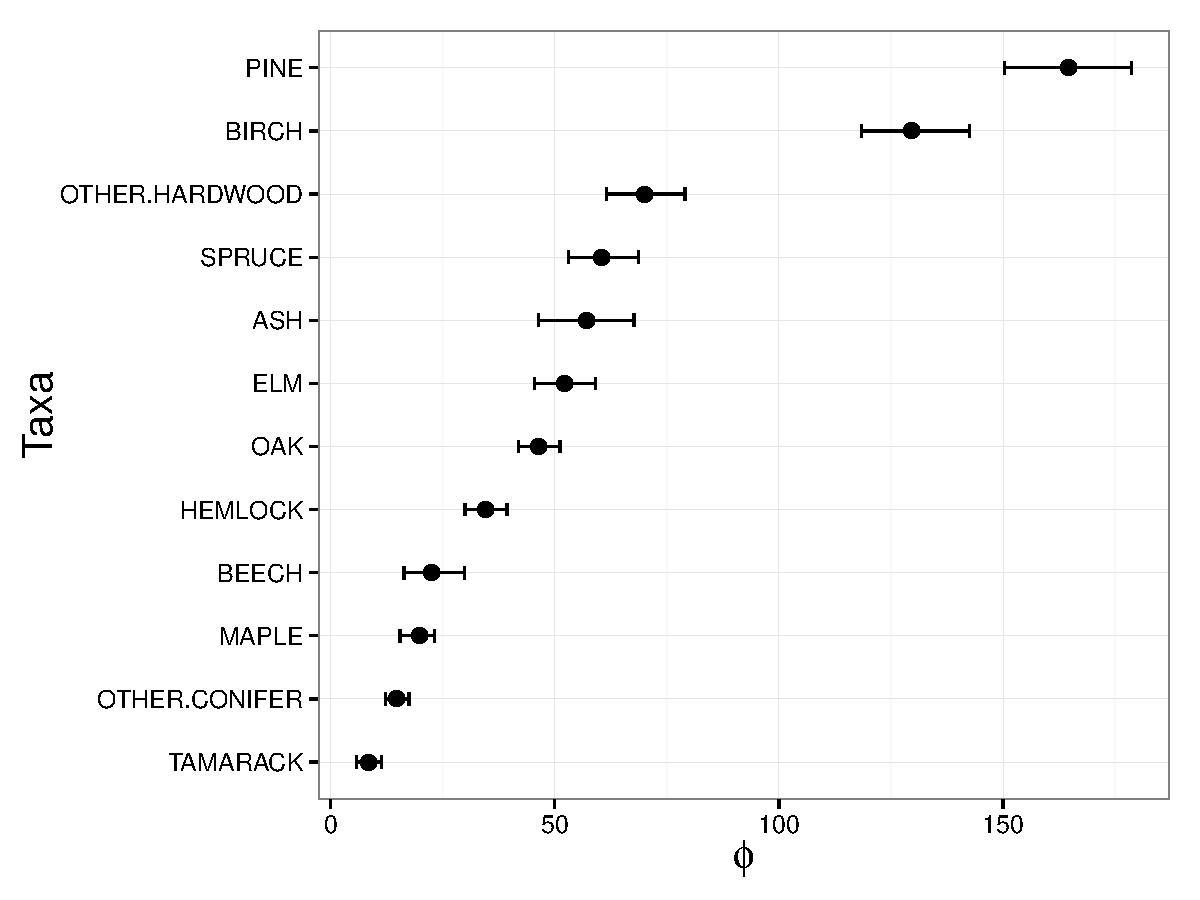
\includegraphics[width=7in]{figures/phi_vary_psi.pdf}
\caption{Mean values of 95\% credible intervals for the estimated values of the differential production parameter $\phi$ for the case where $\psi$ varied by taxon.}
\label{fig:phi_vary_psi}
\end{figure}

%potential pollen maps by taxon
\begin{figure}
\centering
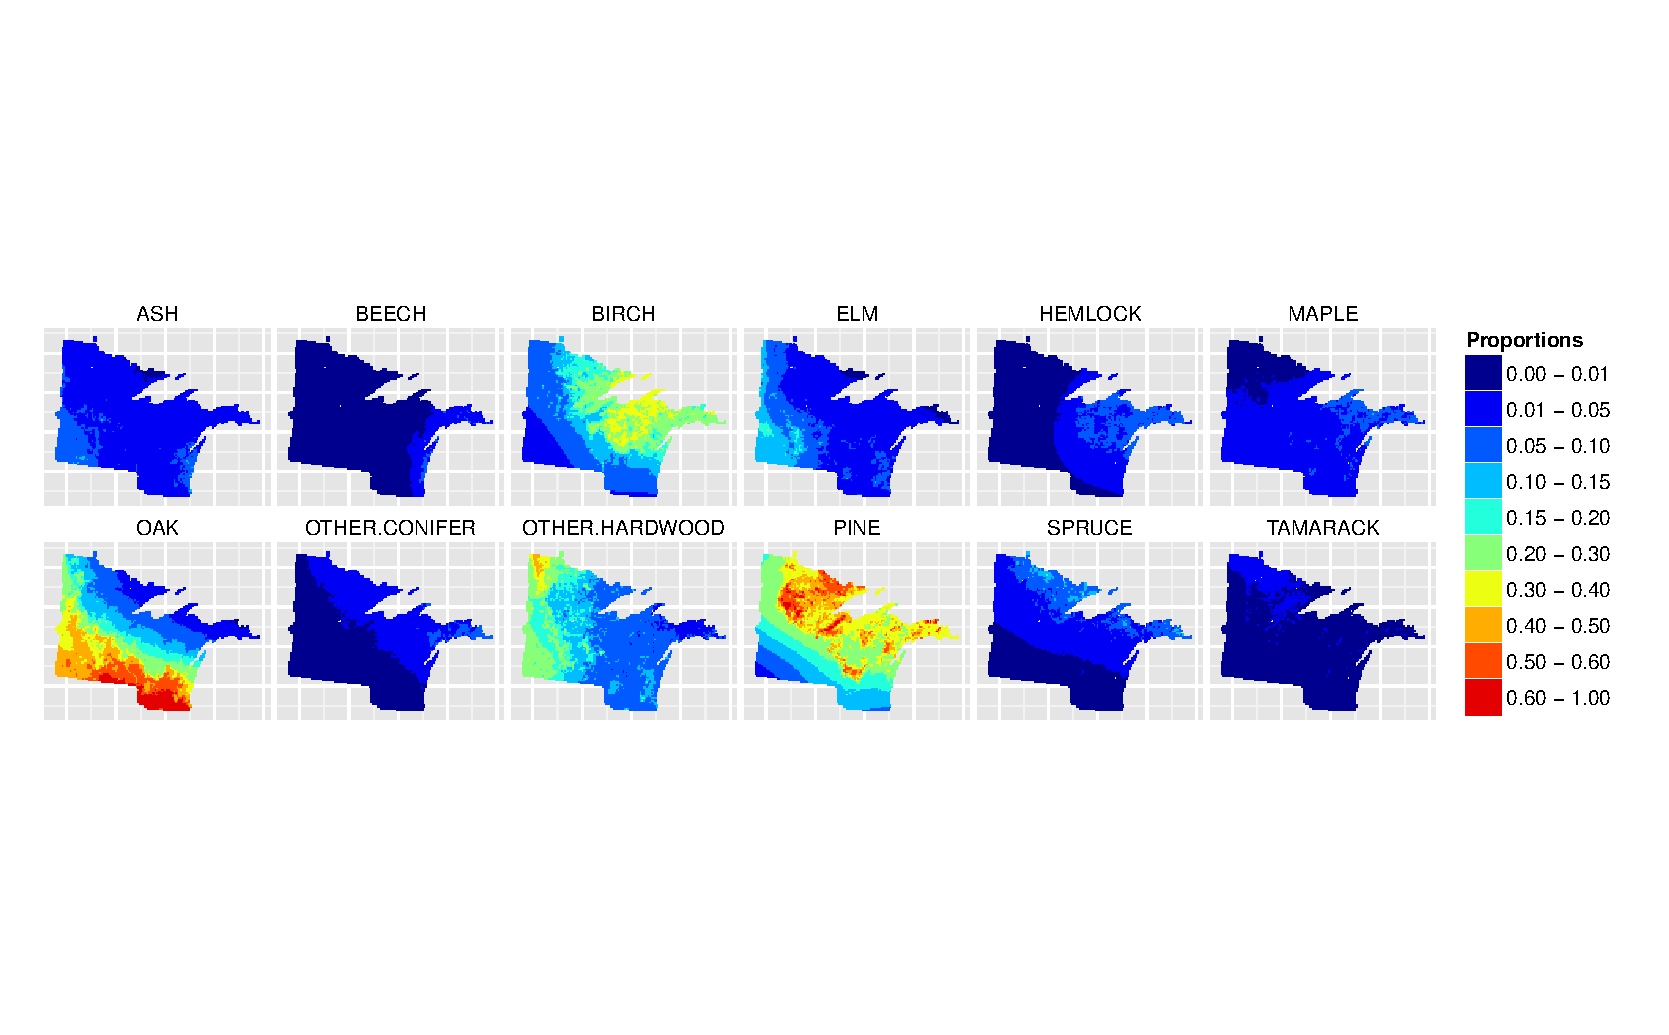
\includegraphics[width=7in]{figures/maps_pollen.pdf}
\caption{Heat maps of model-predicted pollen for each grid cell in the domain, by taxon.}
\label{fig:maps_pollen}
\end{figure}

%PLS data maps by taxon
\begin{figure}
\centering
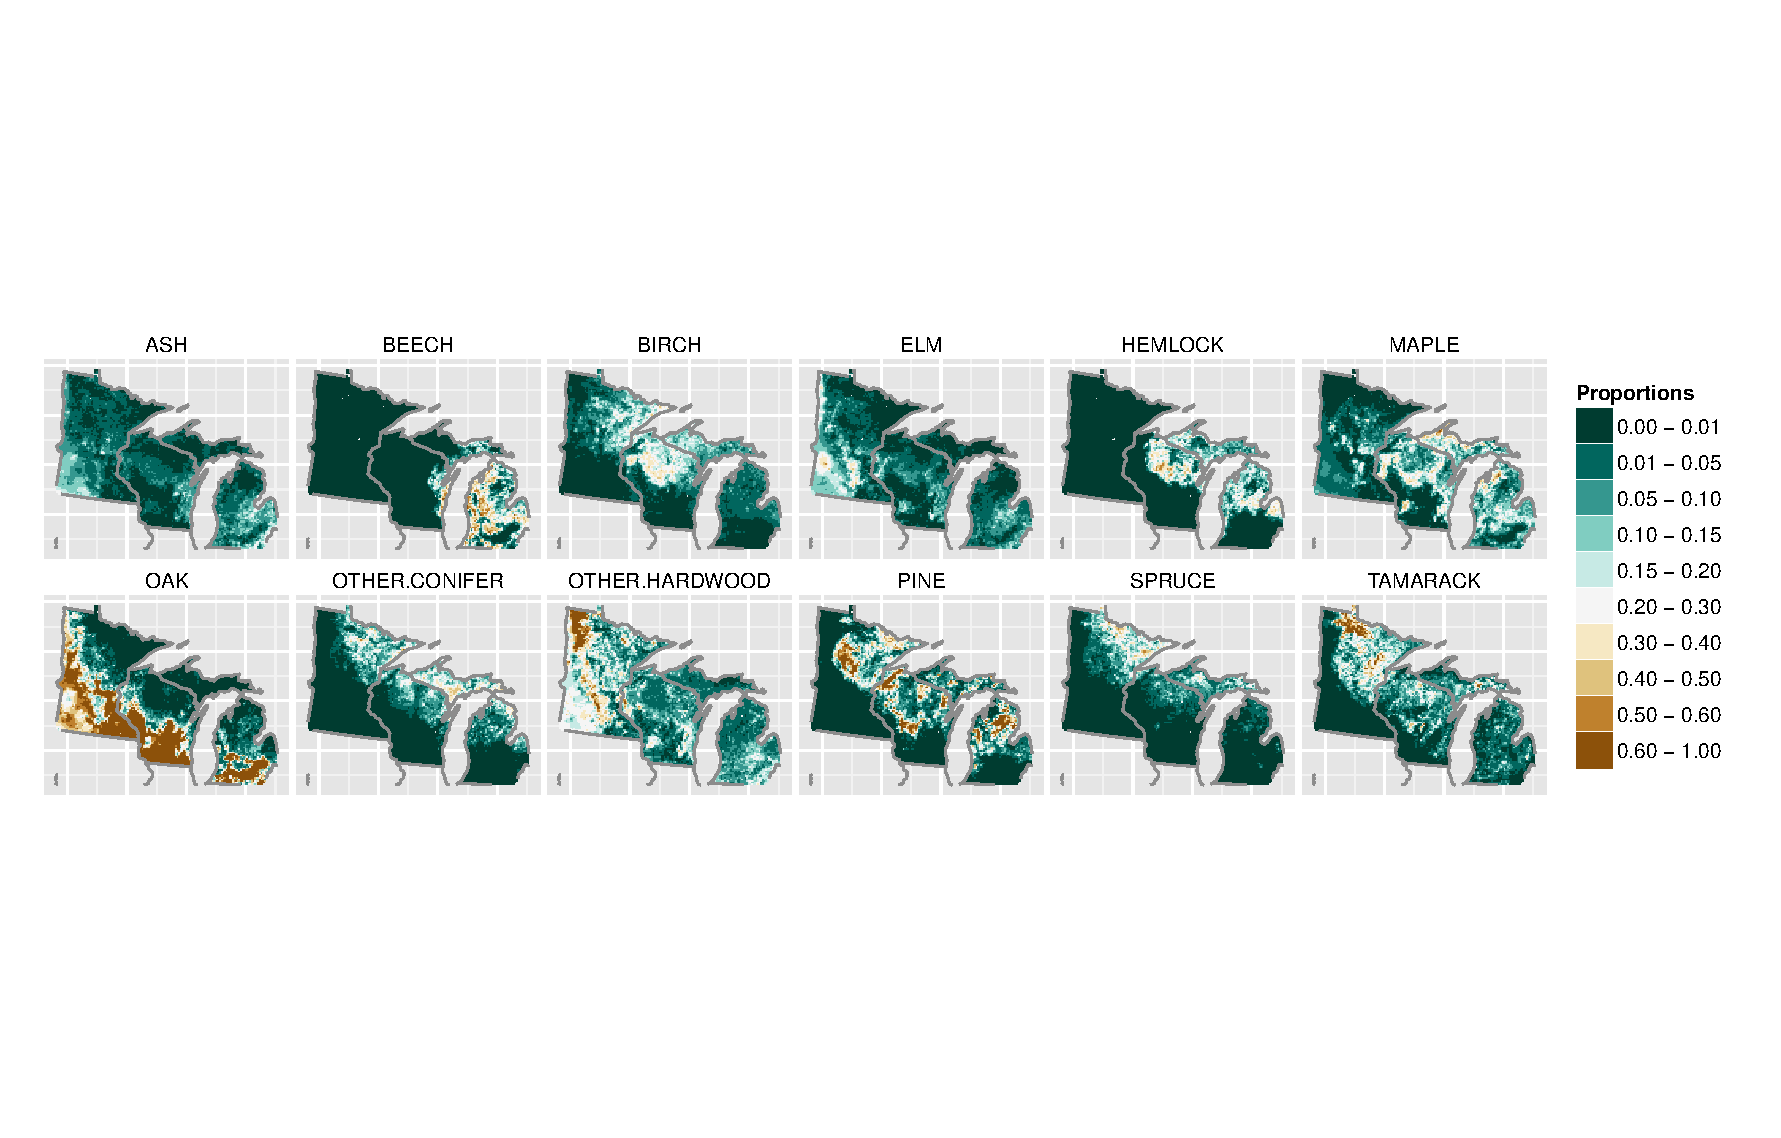
\includegraphics[width=7in]{figures/maps_veg.pdf}
\caption{Heat maps of the PLS data, by taxon.}
\label{fig:maps_pollen}
\end{figure}







\bibliographystyle{plain}
\bibliography{calibration}

\end{document}
